\documentclass[11pt]{article}

% Master file for CPSC 250 lecture notes.
%
% This master file assumes the following directory structure:
%
% LectureNotes/
%     course_notes_master.tex
%     Week1_Lectures/
%         week1a_primitives.pdf
%         week1b_lists_tuples_sets.pdf
%         ...
%     Week2_Lectures/
%         week2a_philosophy_complex_objects.pdf
%         ...
%     Week3_Lectures/
%         week3a_derived_classes.pdf
%         ...
%     Week4_Lectures/
%         week4a_more_on_fibonacci.pdf
%         ...
%
% Because the individual lecture notes are standalone LaTeX documents,
% this master file includes the compiled PDFs rather than \input-ing
% the .tex files directly.

\usepackage[margin=1in]{geometry}
\usepackage{pdfpages}
\usepackage{hyperref}

\hypersetup{
    colorlinks=true,
    linkcolor=blue,
    urlcolor=blue
}

\title{CPSC 250 \\ Programming for Data Manipulation \\ Complete Lecture Notes}
\author{Edward Brash}
\date{}

\begin{document}

\maketitle
\tableofcontents
\clearpage

% ============================================================
% Week 1
% ============================================================

\section*{Week 1: Python Review and Core Data Structures}
\addcontentsline{toc}{section}{Week 1: Python Review and Core Data Structures}

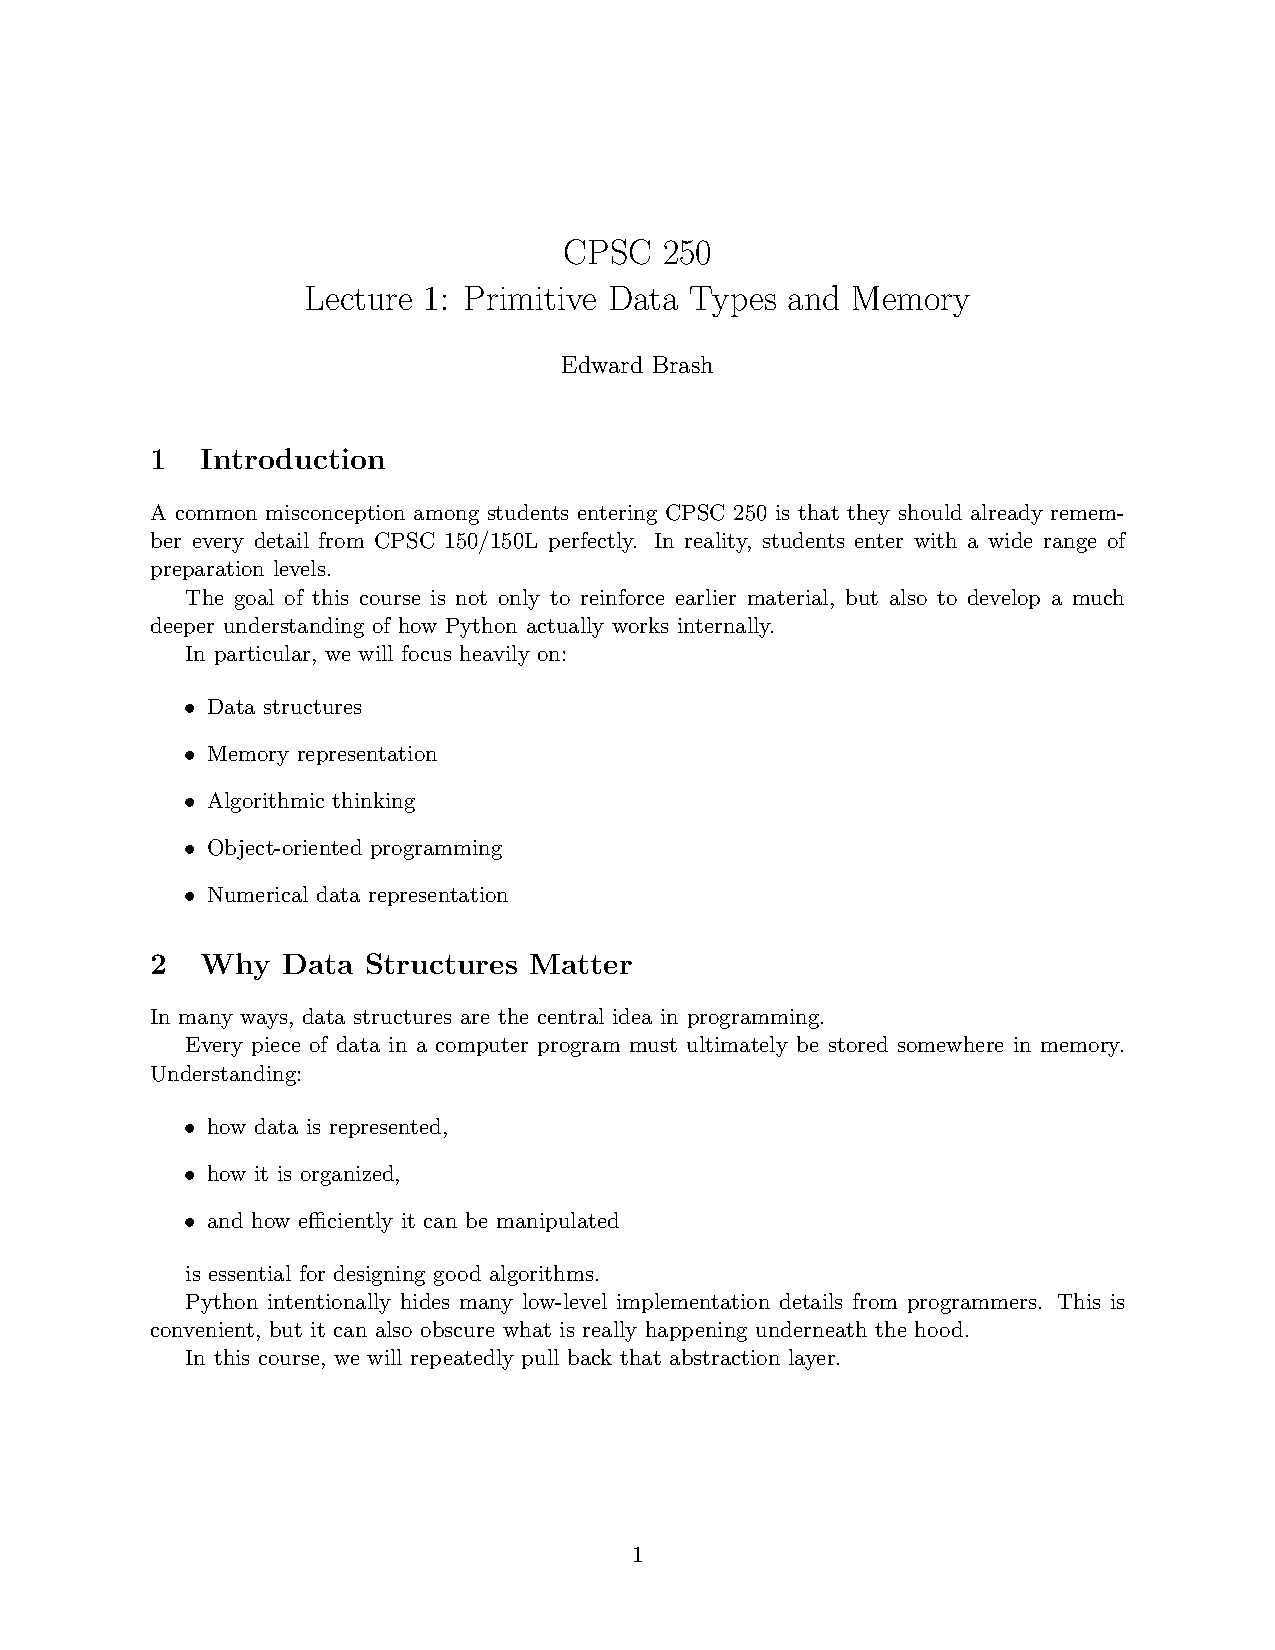
\includepdf[
    pages=-,
    addtotoc={1,subsection,2,{Primitive Data Types},week1a}
]{Week1_Lectures/week1a_primitives.pdf}

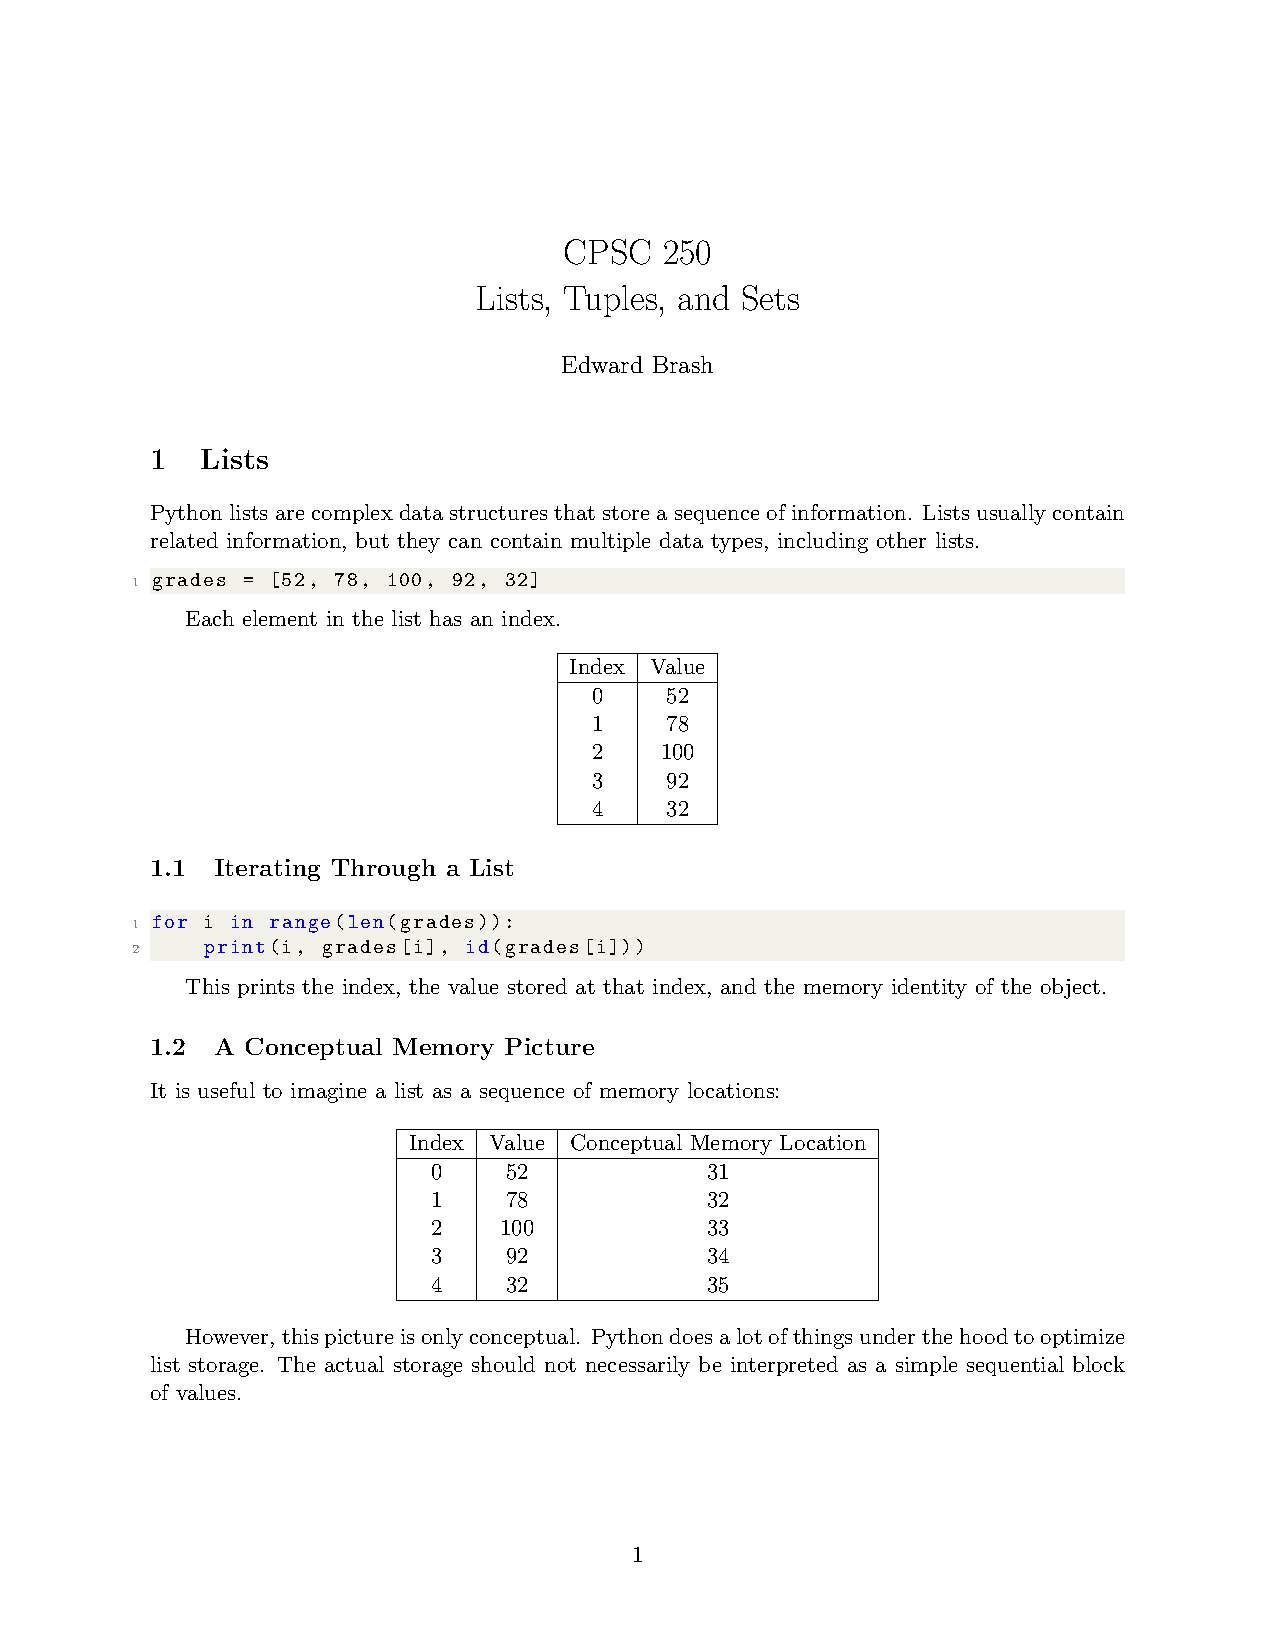
\includepdf[
    pages=-,
    addtotoc={1,subsection,2,{Lists, Tuples, and Sets},week1b}
]{Week1_Lectures/week1b_lists_tuples_sets.pdf}

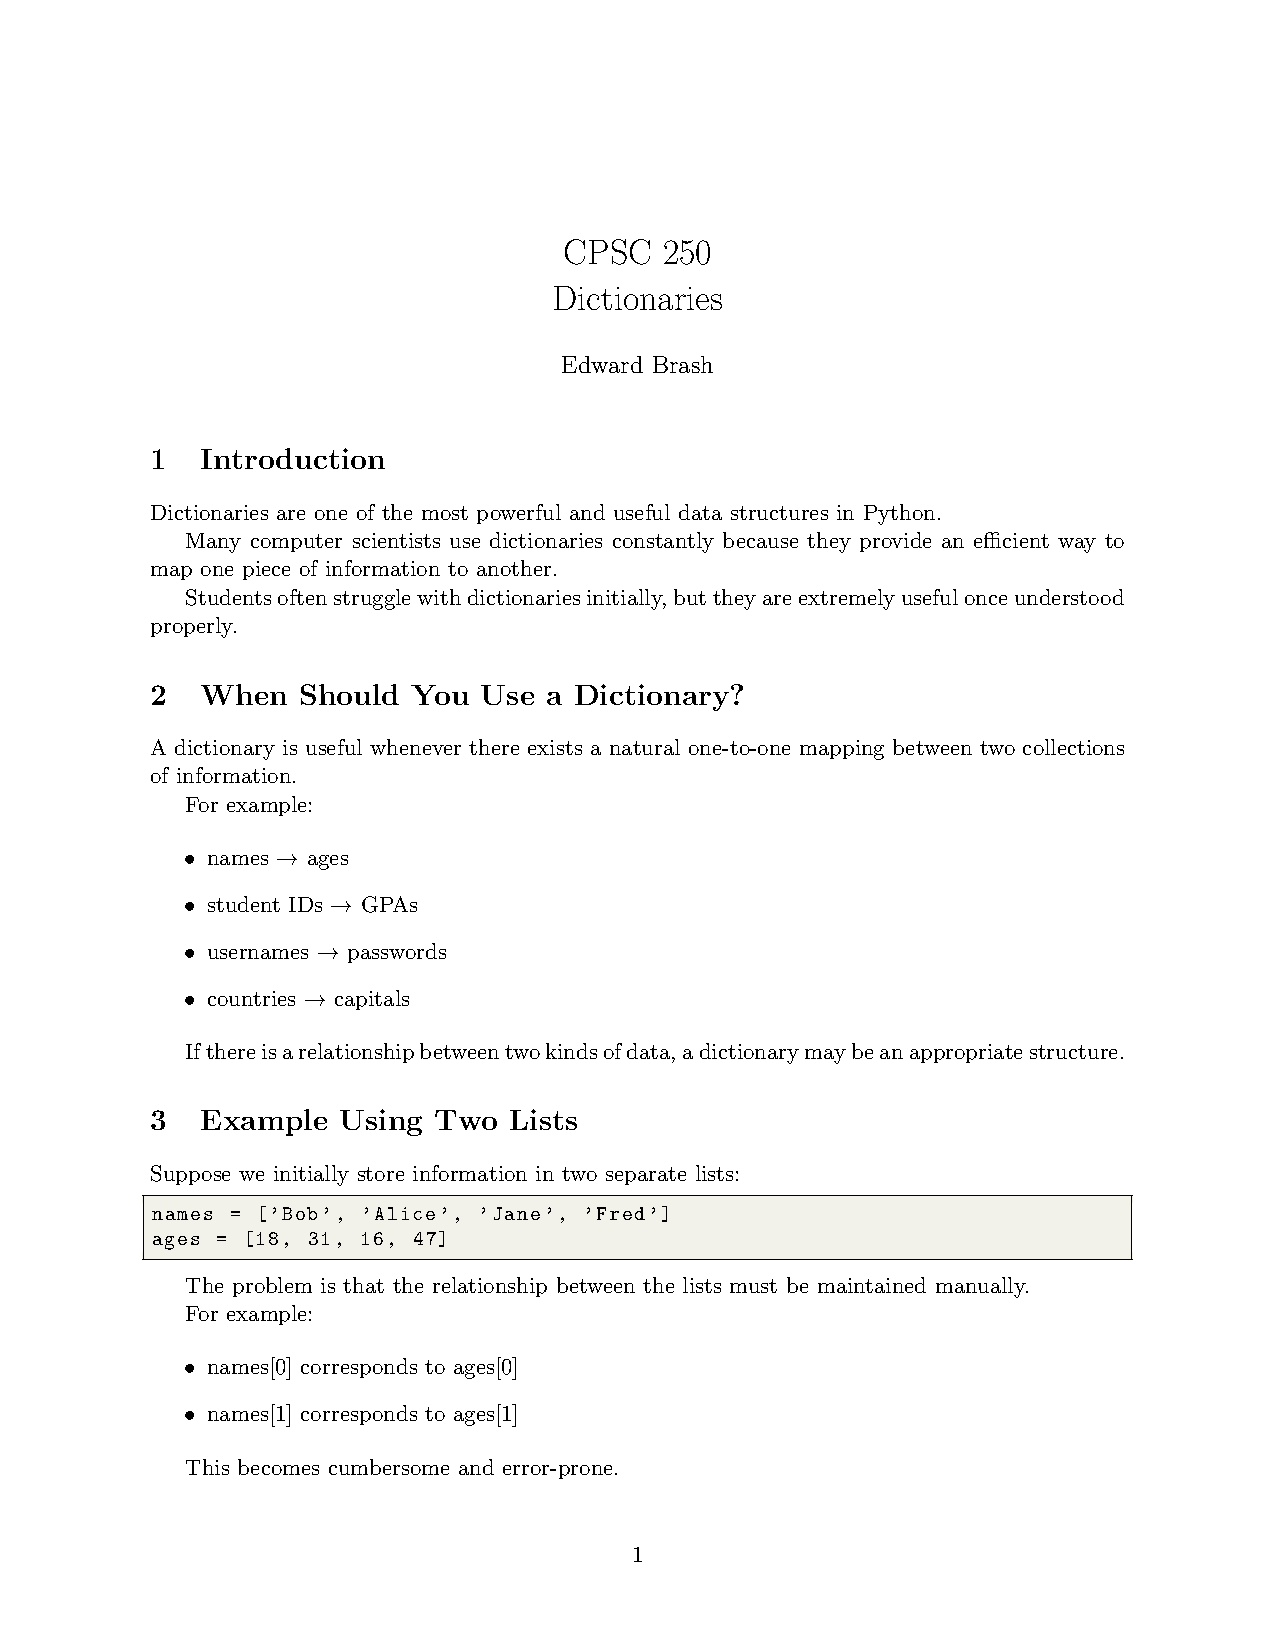
\includepdf[
    pages=-,
    addtotoc={1,subsection,2,{Dictionaries},week1c}
]{Week1_Lectures/week1c_dicts.pdf}

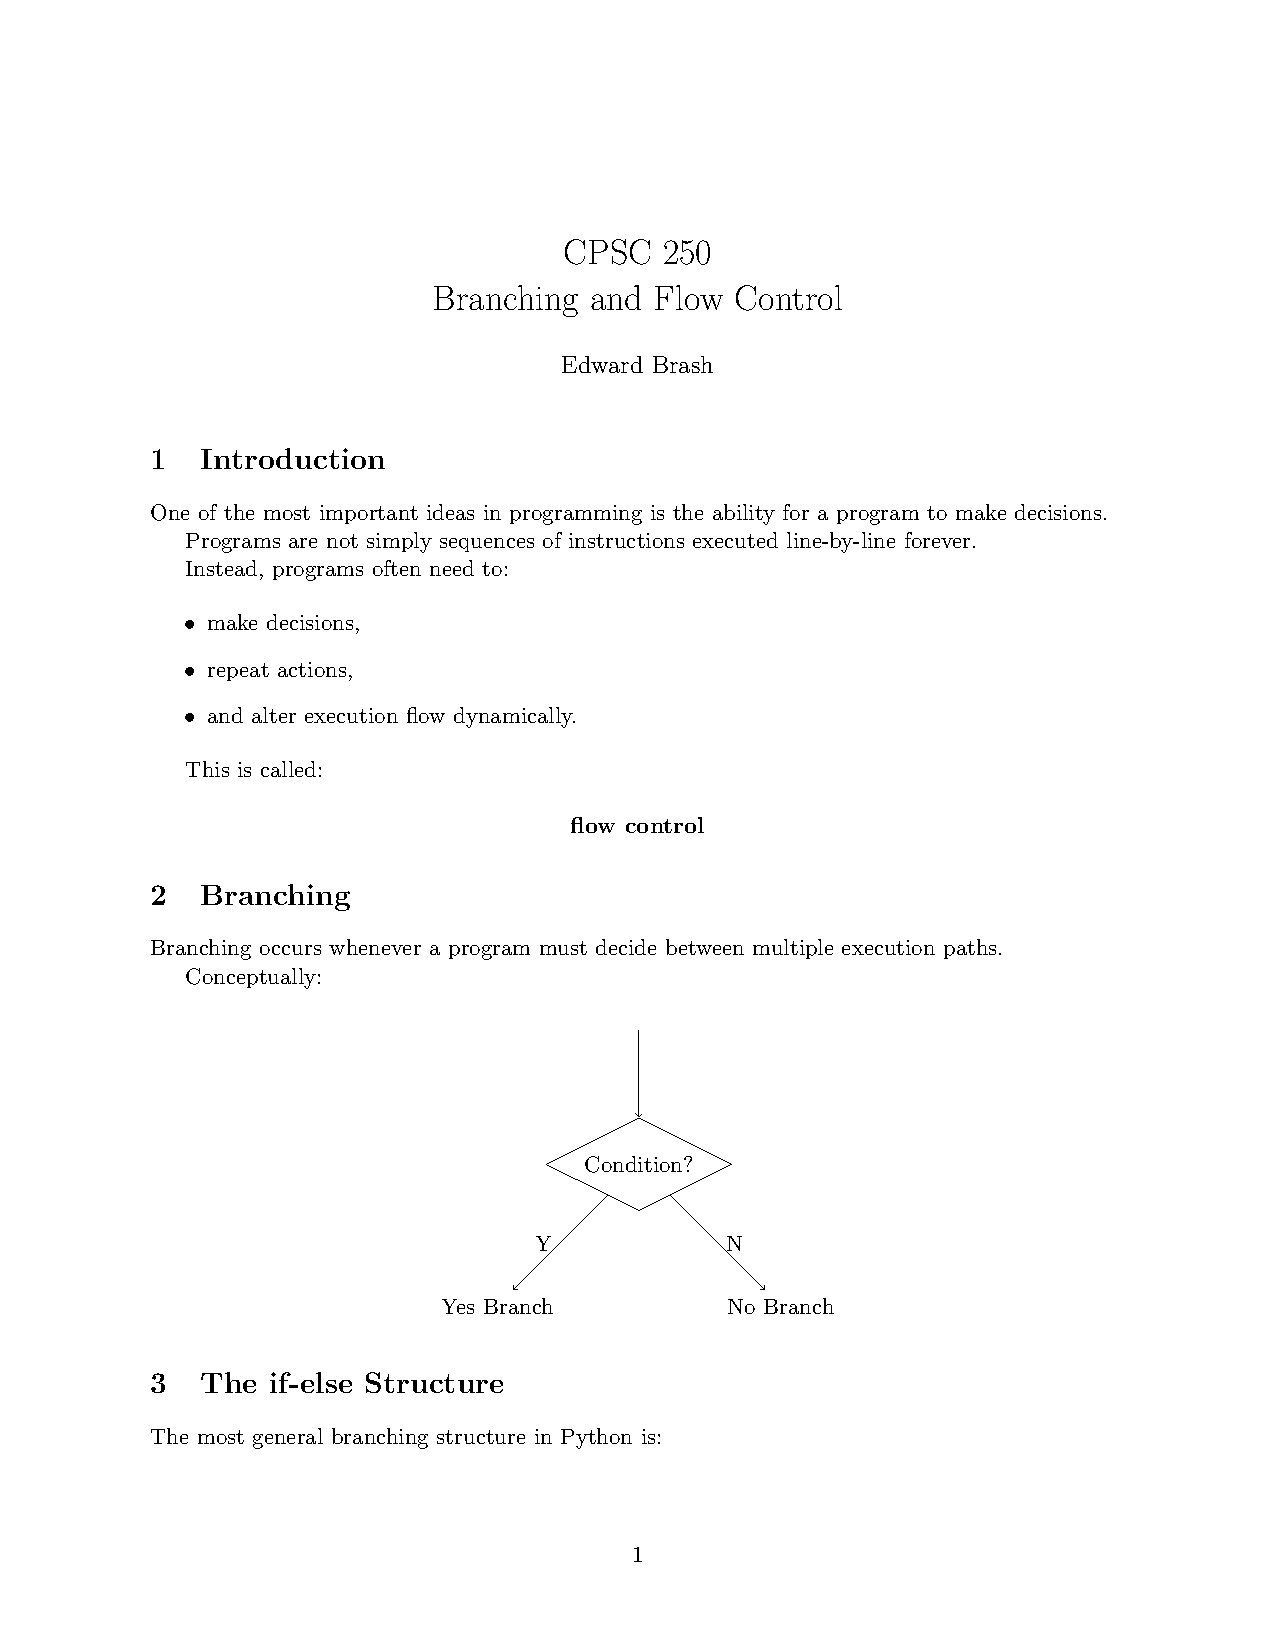
\includepdf[
    pages=-,
    addtotoc={1,subsection,2,{Branching and Flow Control},week1d}
]{Week1_Lectures/week1d_branching.pdf}

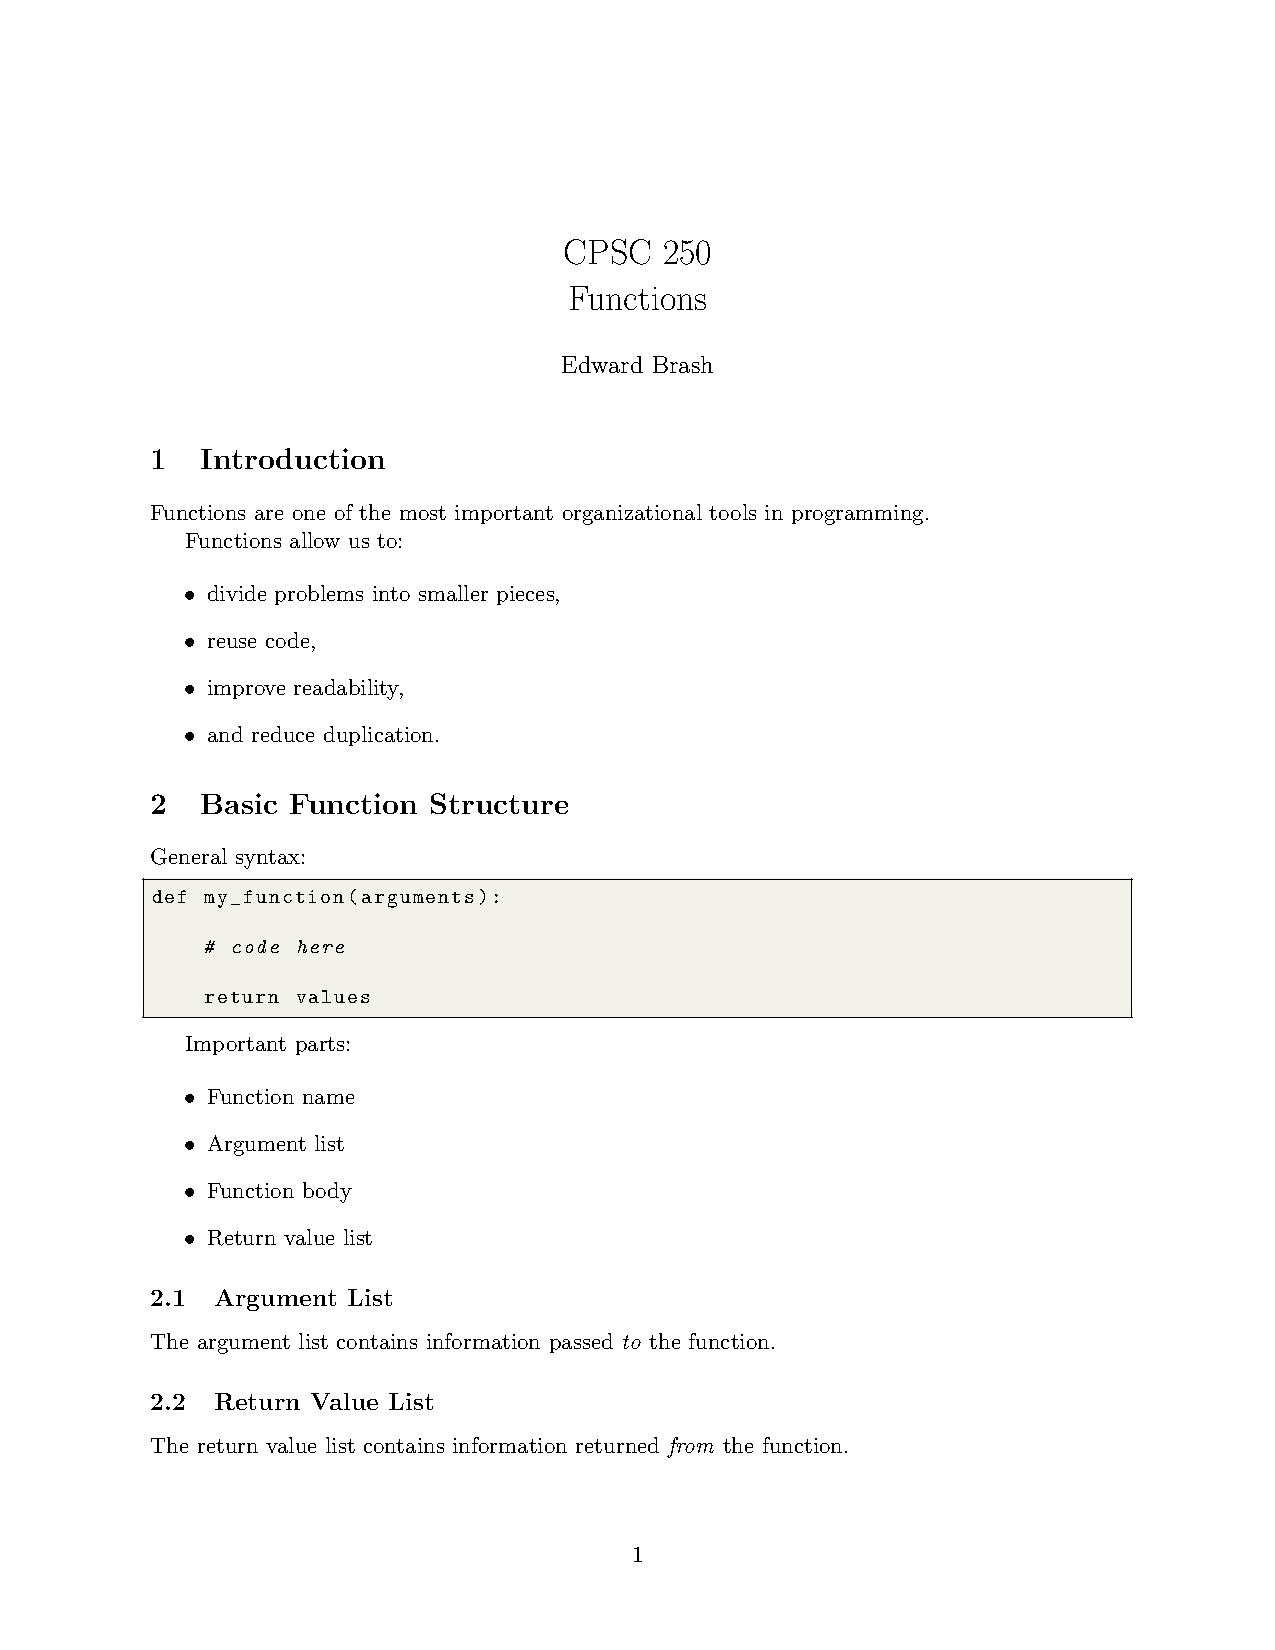
\includepdf[
    pages=-,
    addtotoc={1,subsection,2,{Functions},week1e}
]{Week1_Lectures/week1e_functions.pdf}

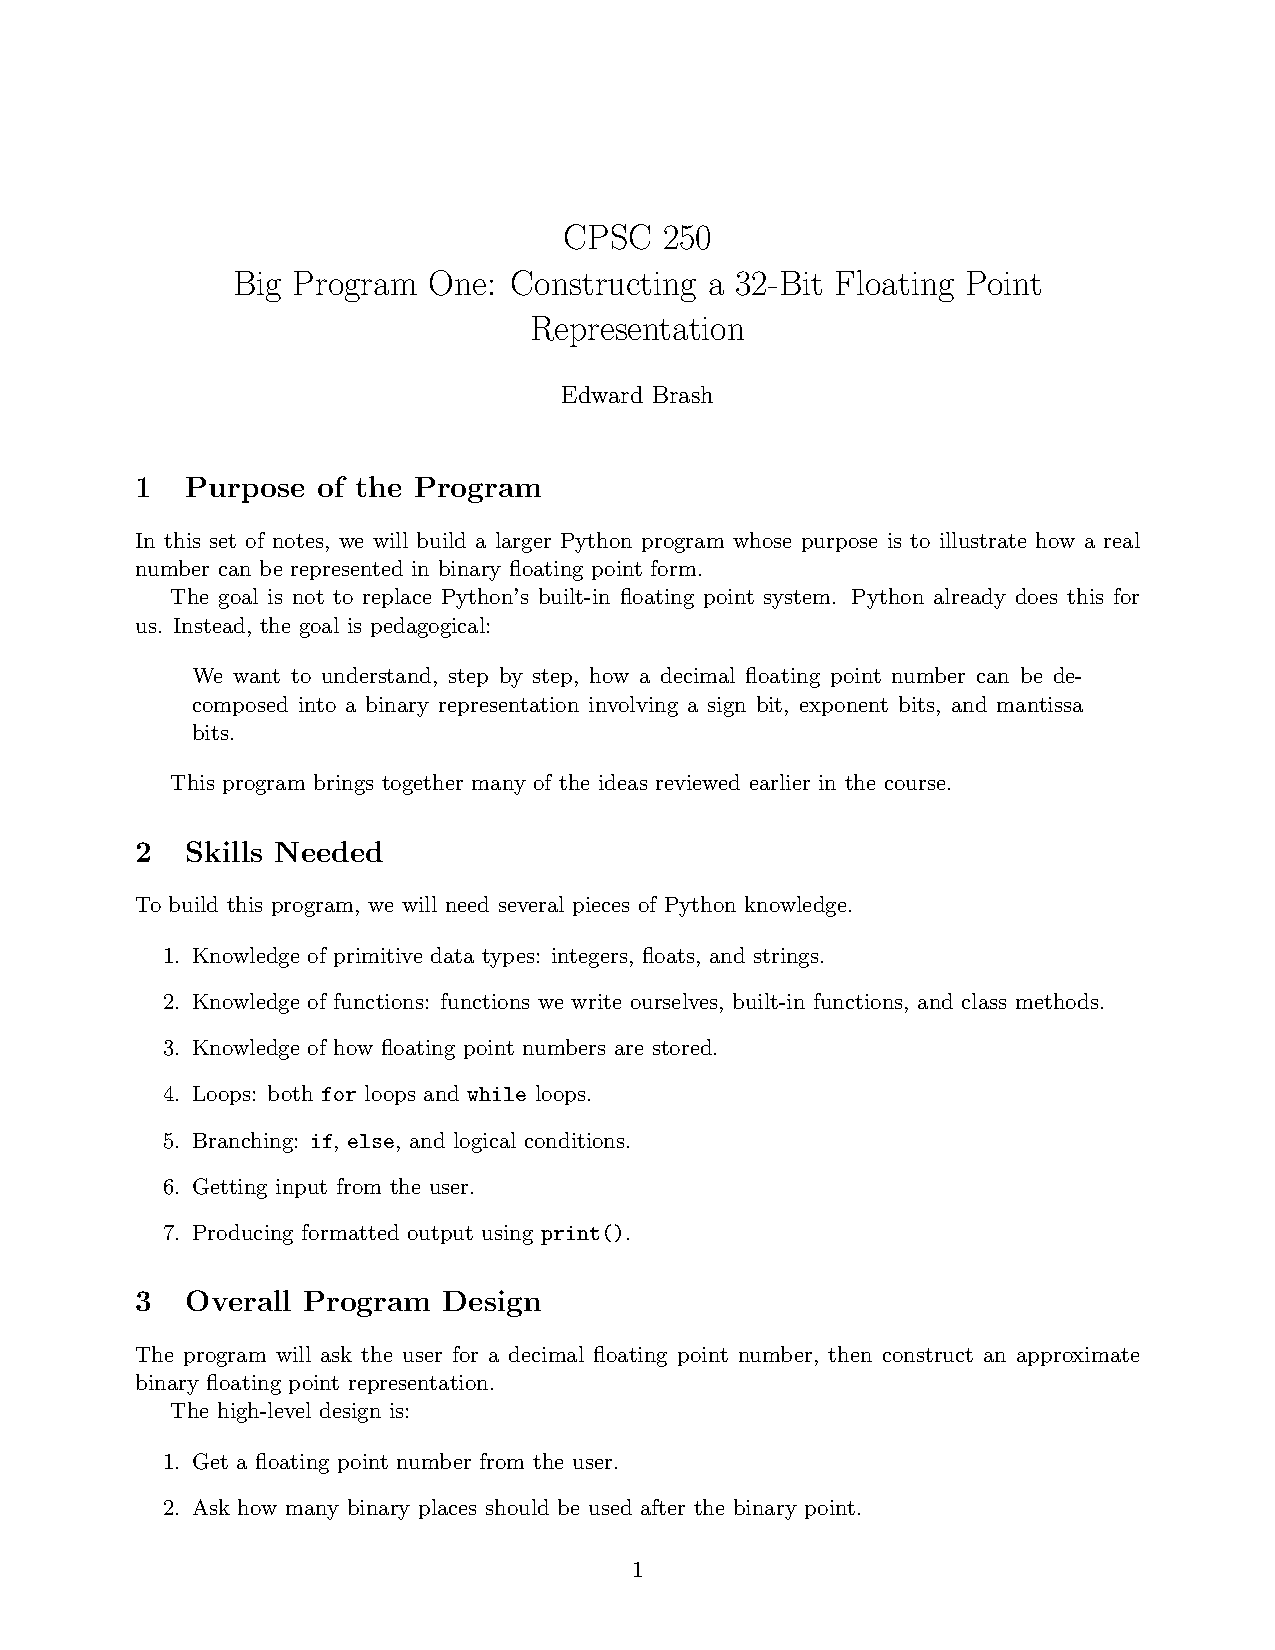
\includepdf[
    pages=-,
    addtotoc={1,subsection,2,{Big Program One},week1f}
]{Week1_Lectures/week1f_big_program_one.pdf}

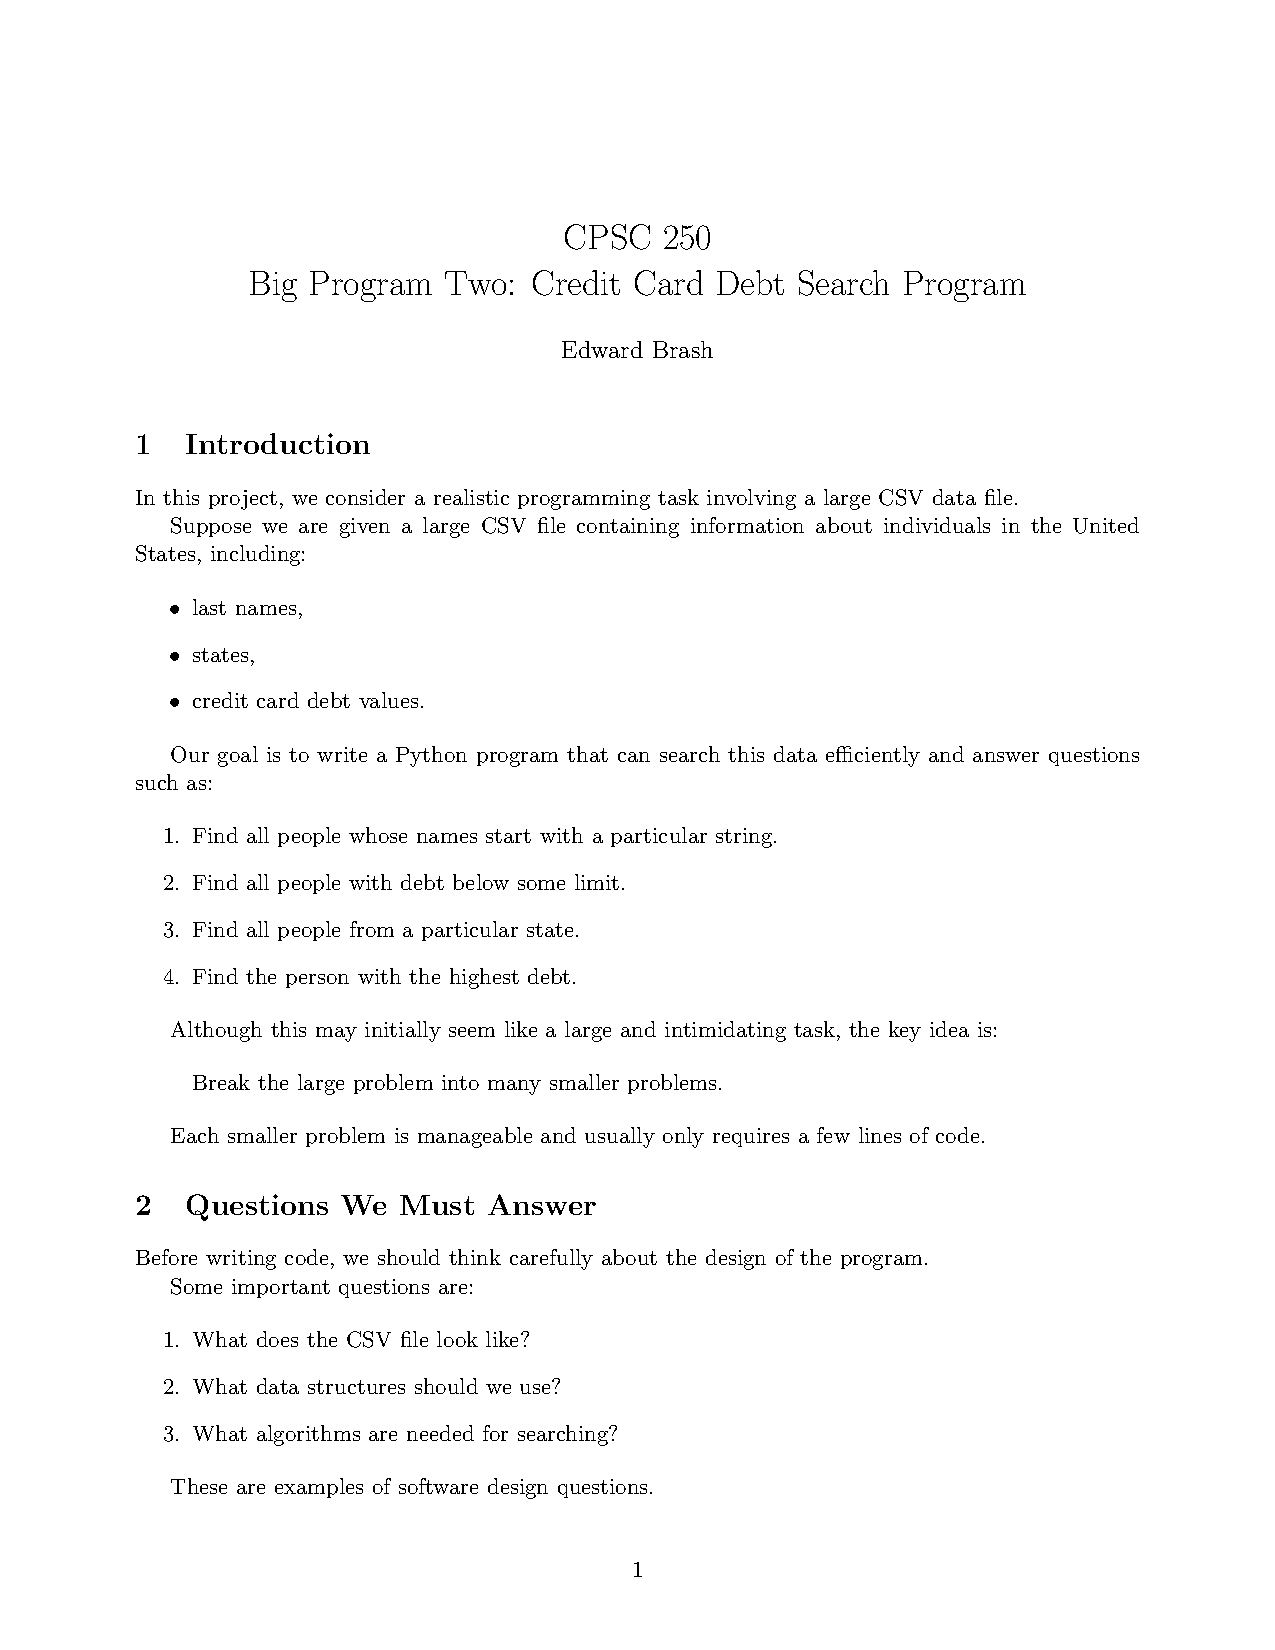
\includepdf[
    pages=-,
    addtotoc={1,subsection,2,{Big Program Two},week1g}
]{Week1_Lectures/week1g_big_program_two.pdf}

% ============================================================
% Week 2
% ============================================================

\clearpage
\section*{Week 2: Object-Oriented Programming}
\addcontentsline{toc}{section}{Week 2: Object-Oriented Programming}

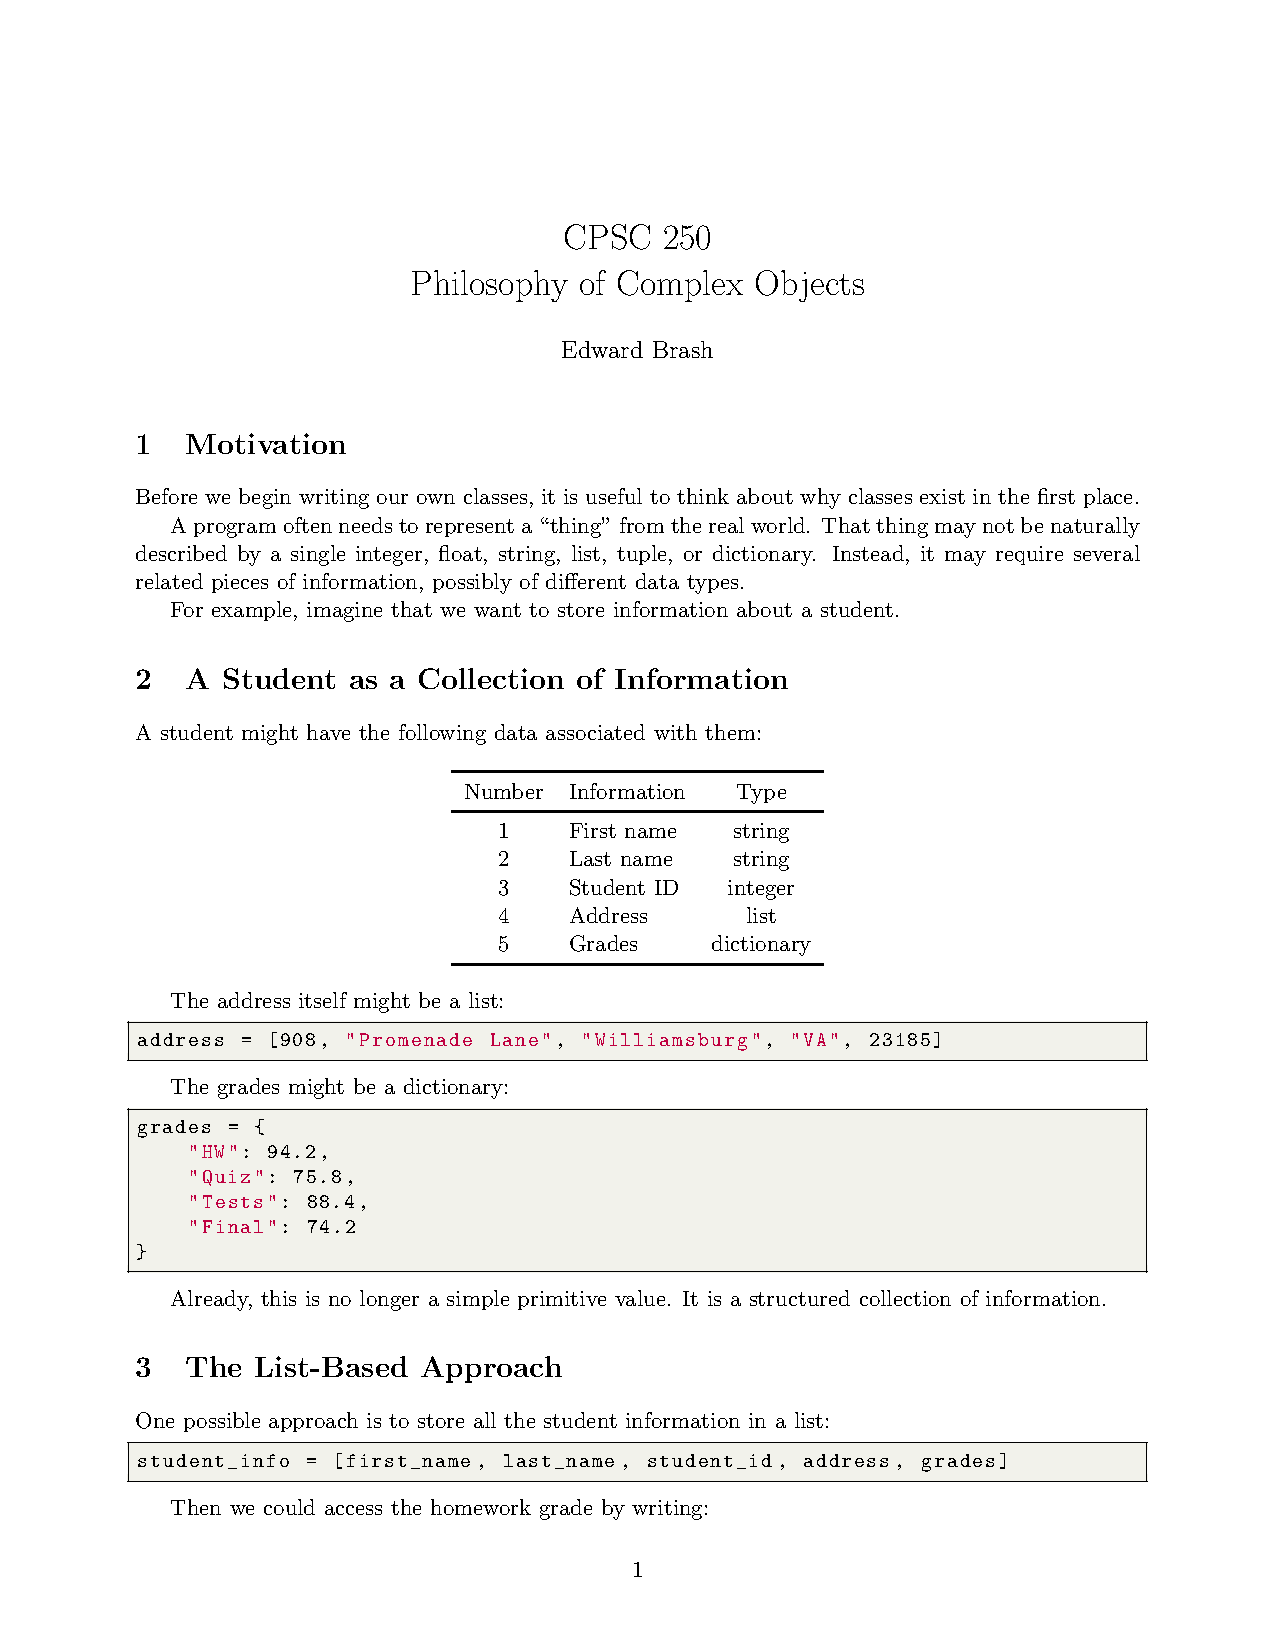
\includepdf[
    pages=-,
    addtotoc={1,subsection,2,{Philosophy of Complex Objects},week2a}
]{Week2_Lectures/week2a_philosophy_complex_objects.pdf}

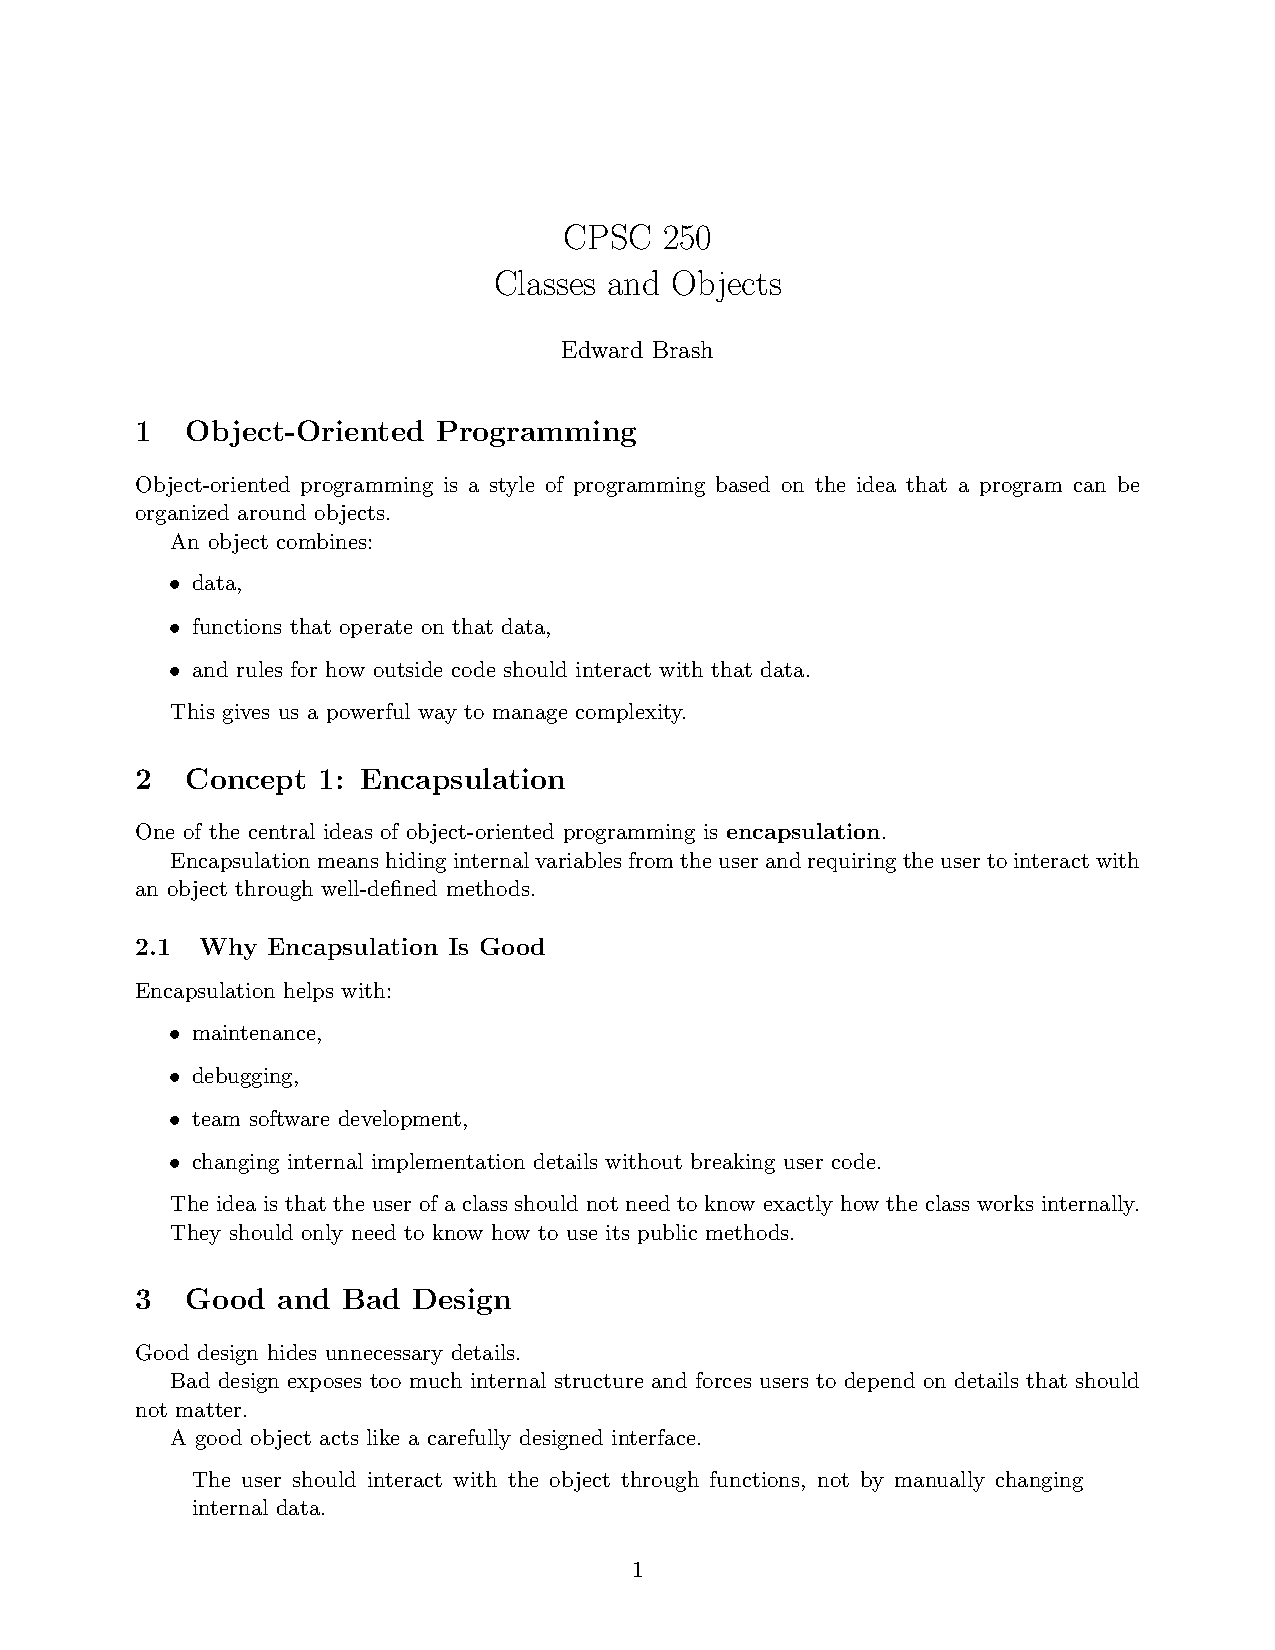
\includepdf[
    pages=-,
    addtotoc={1,subsection,2,{Classes and Objects},week2b}
]{Week2_Lectures/week2b_classes_objects.pdf}

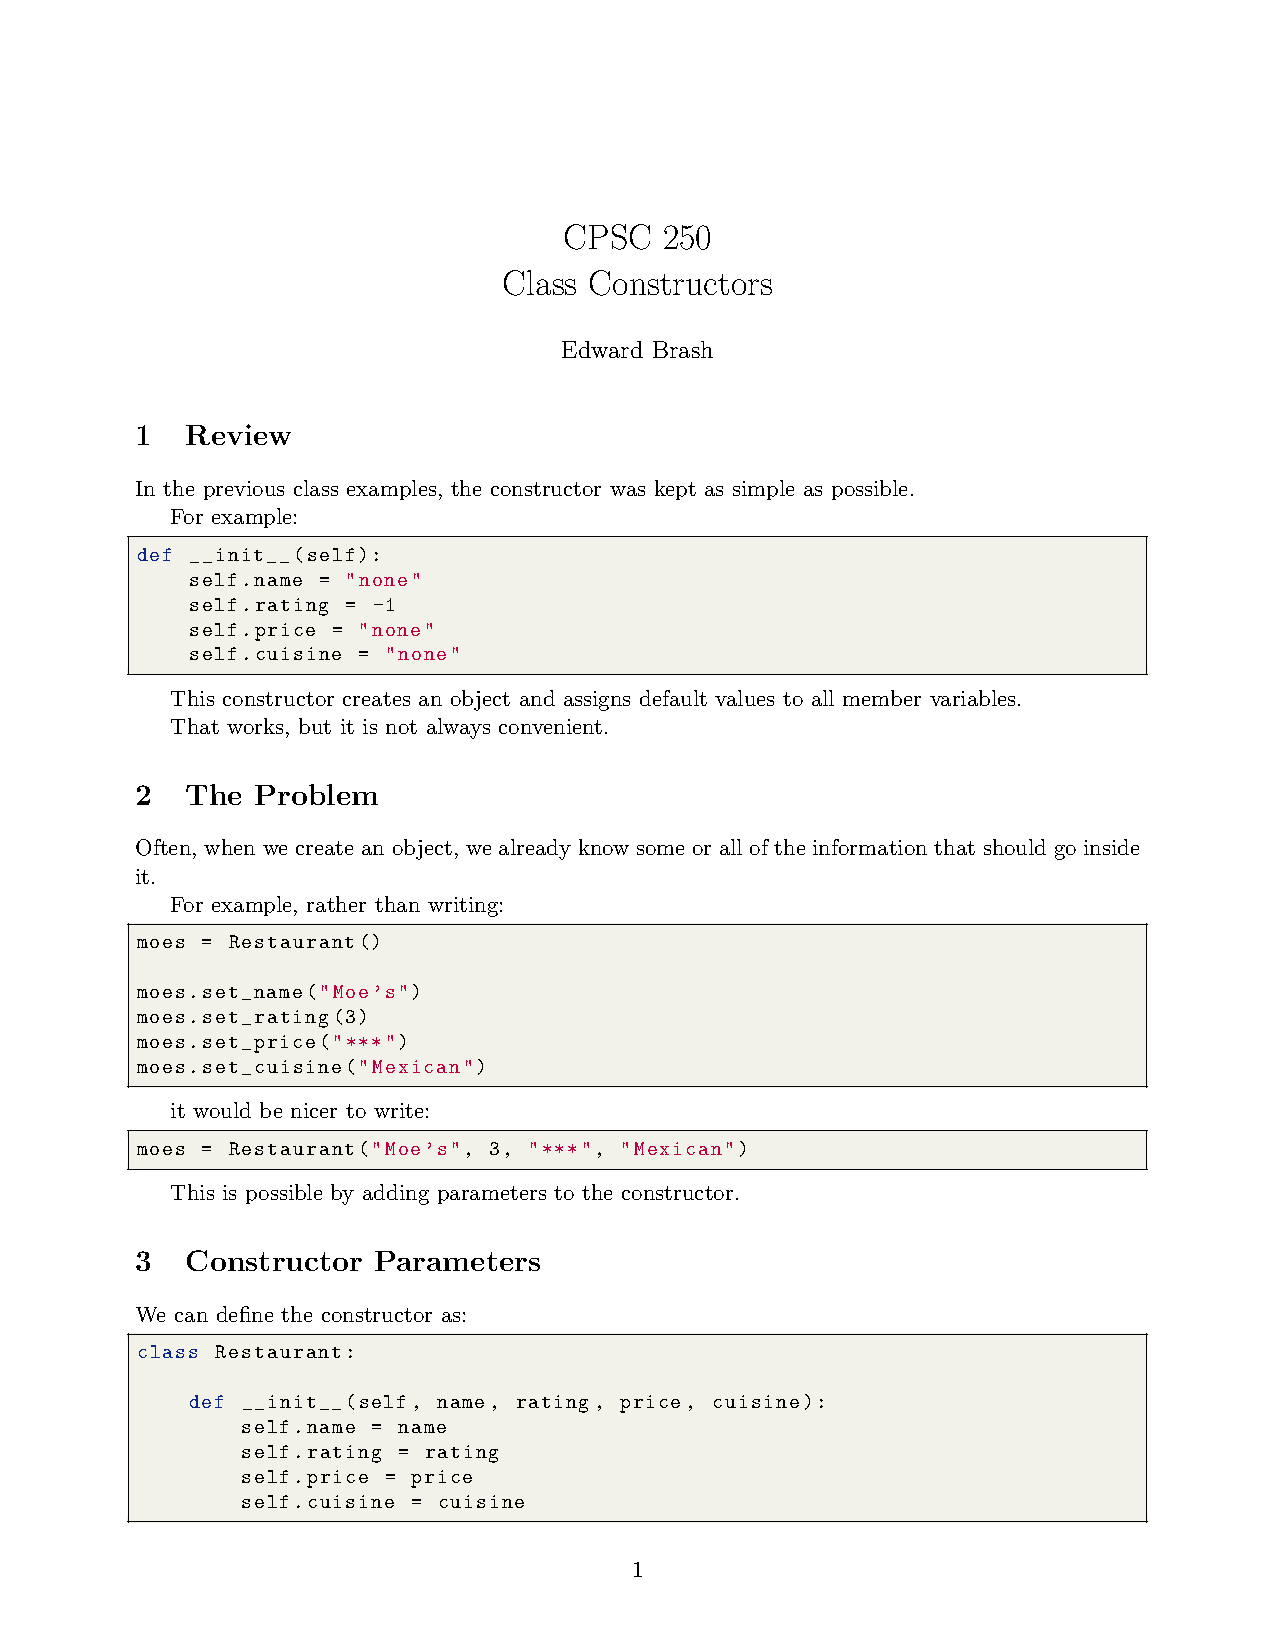
\includepdf[
    pages=-,
    addtotoc={1,subsection,2,{Class Constructors},week2c}
]{Week2_Lectures/week2c_class_constructors.pdf}

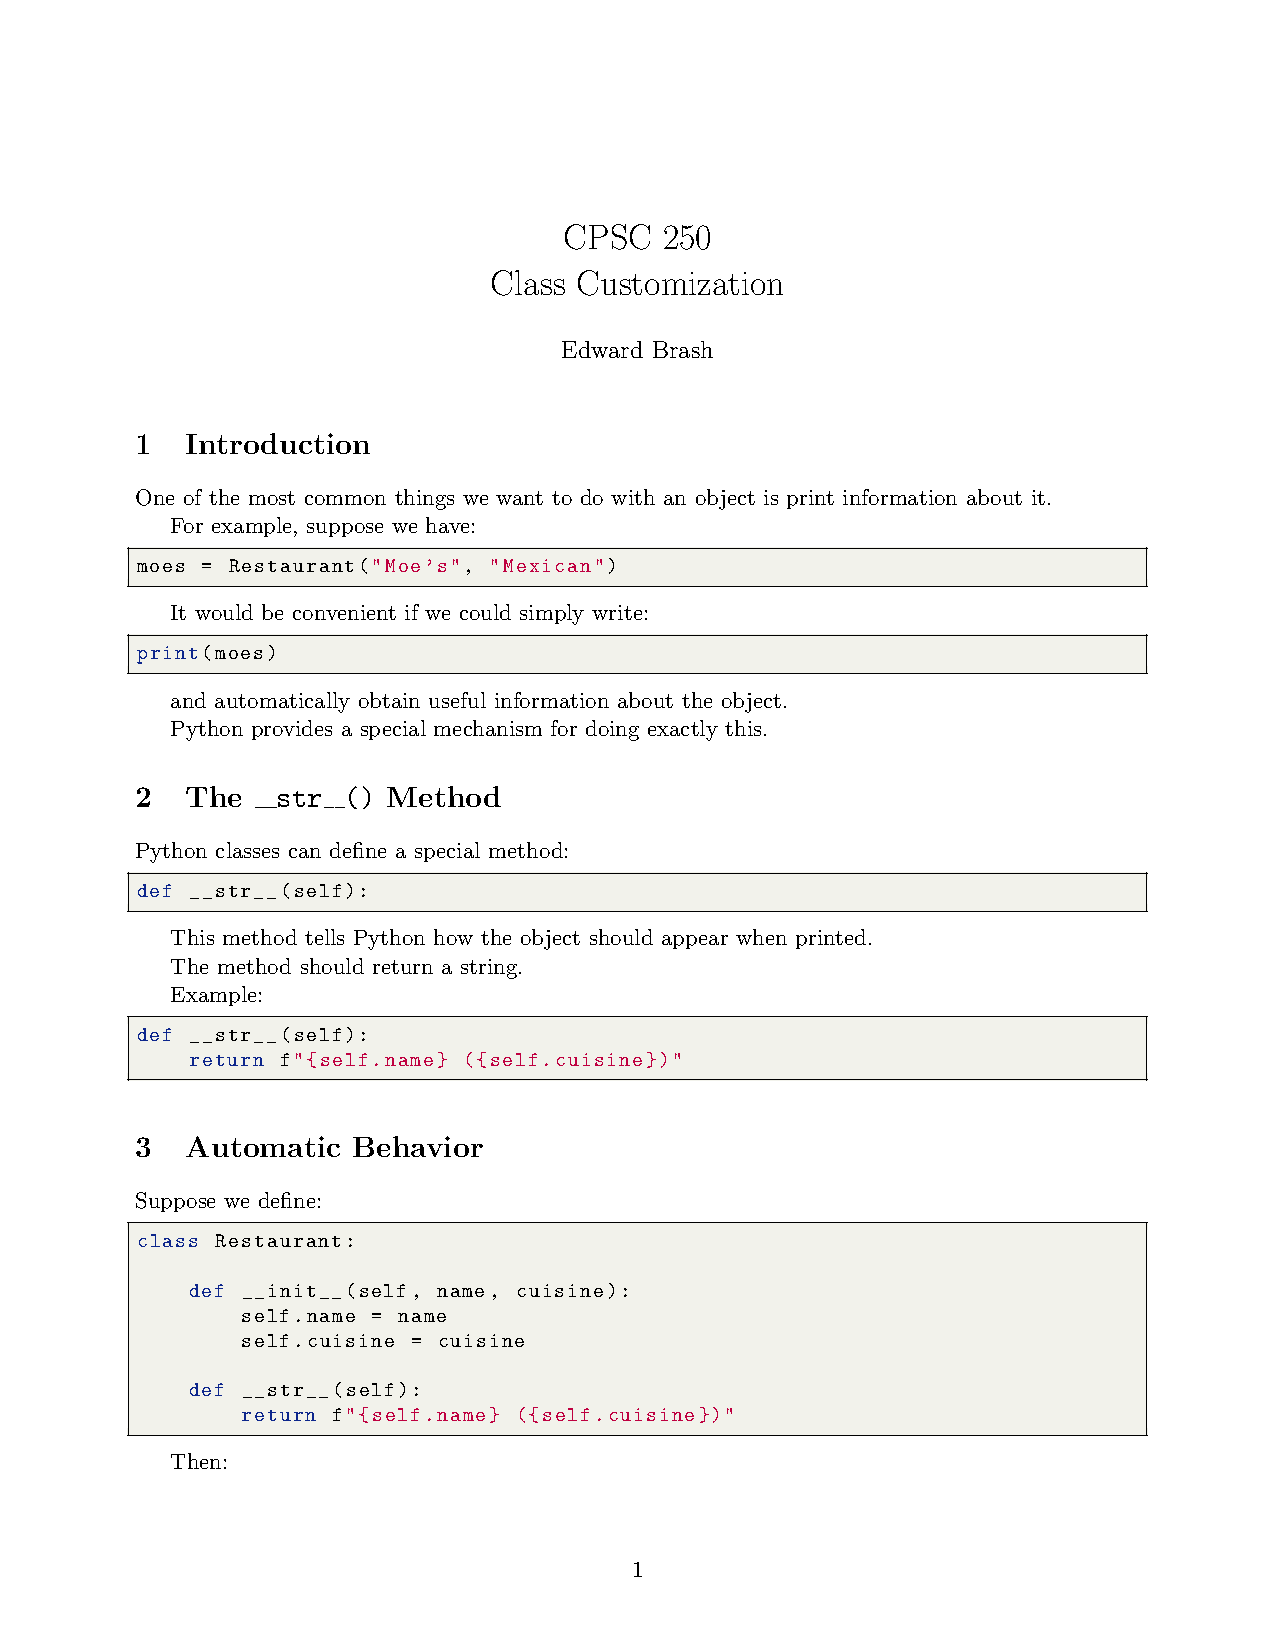
\includepdf[
    pages=-,
    addtotoc={1,subsection,2,{Class Customization},week2d}
]{Week2_Lectures/week2d_class_customization.pdf}

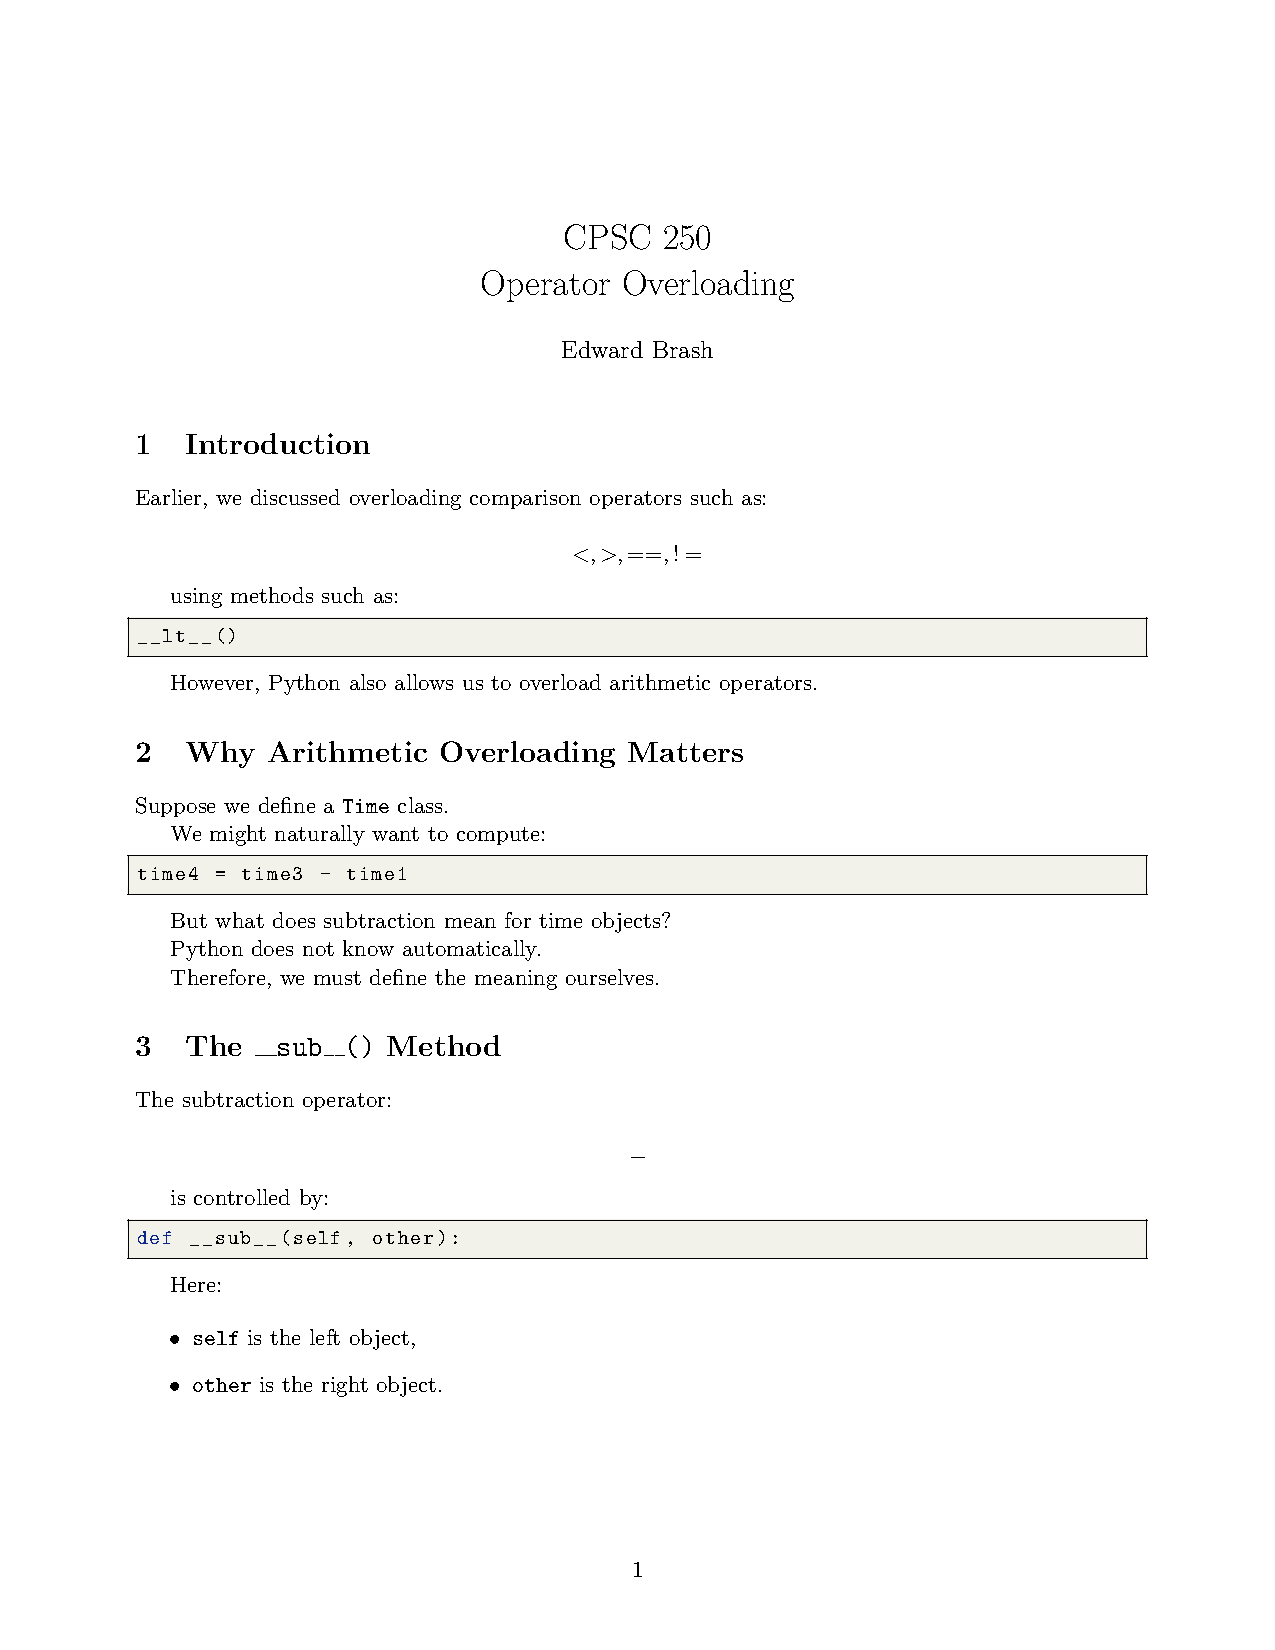
\includepdf[
    pages=-,
    addtotoc={1,subsection,2,{Operator Overloading},week2e}
]{Week2_Lectures/week2e_operator_overloading.pdf}

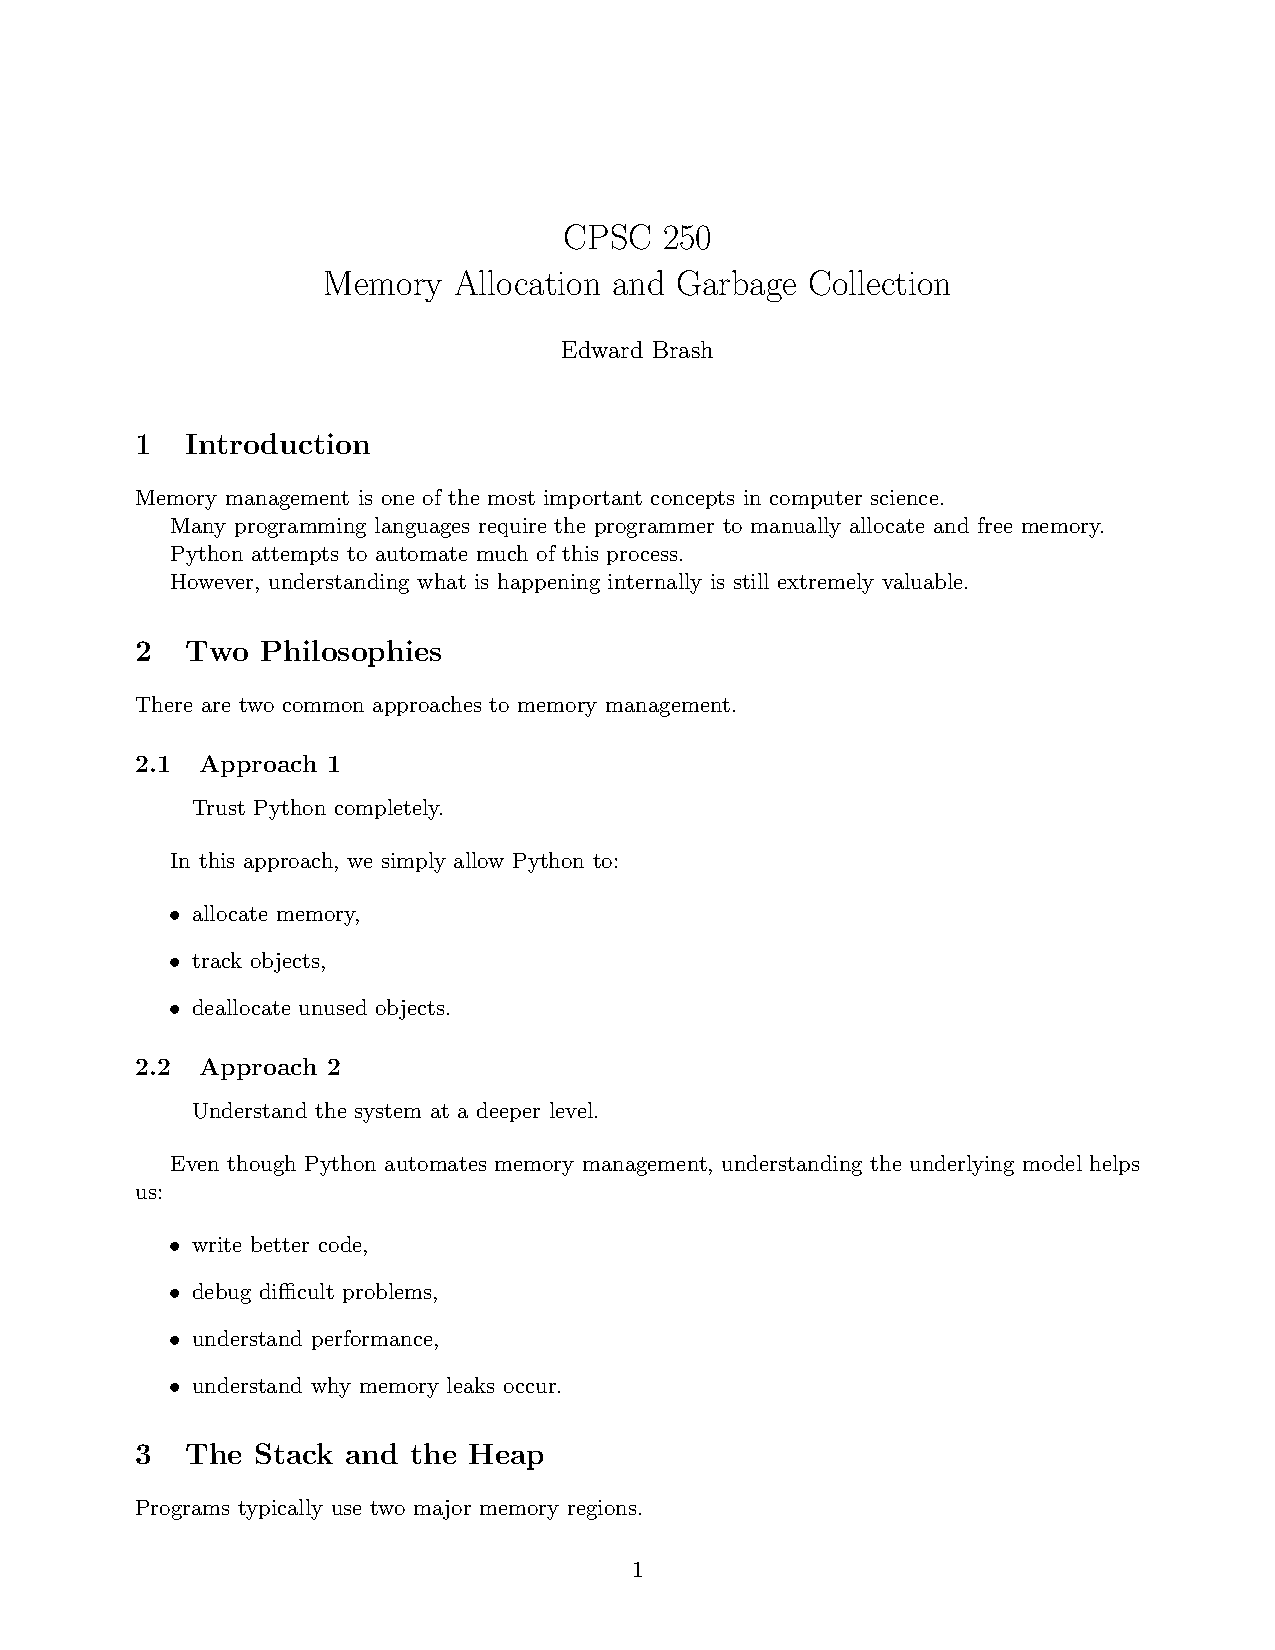
\includepdf[
    pages=-,
    addtotoc={1,subsection,2,{Memory Allocation},week2f}
]{Week2_Lectures/week2f_memory_allocation.pdf}

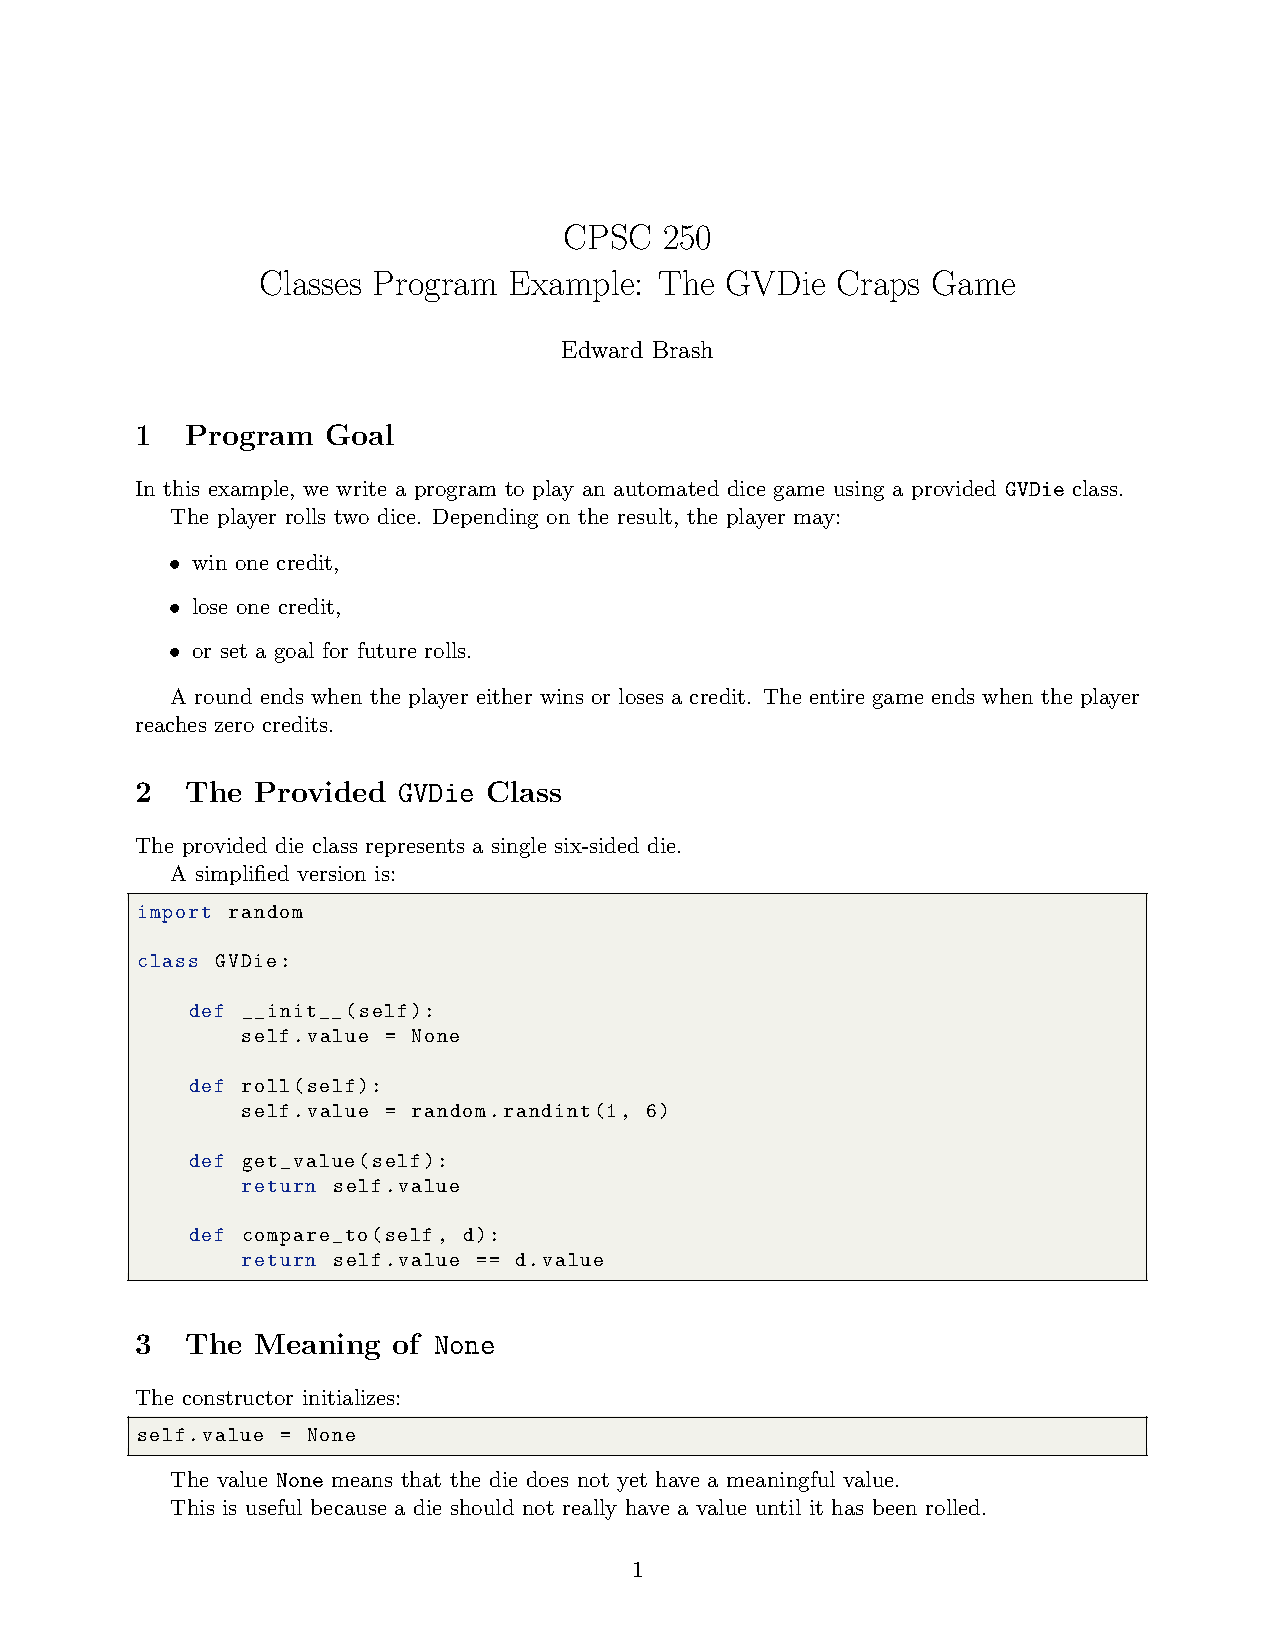
\includepdf[
    pages=-,
    addtotoc={1,subsection,2,{Classes Program Example},week2g}
]{Week2_Lectures/week2g_classes_program_example.pdf}

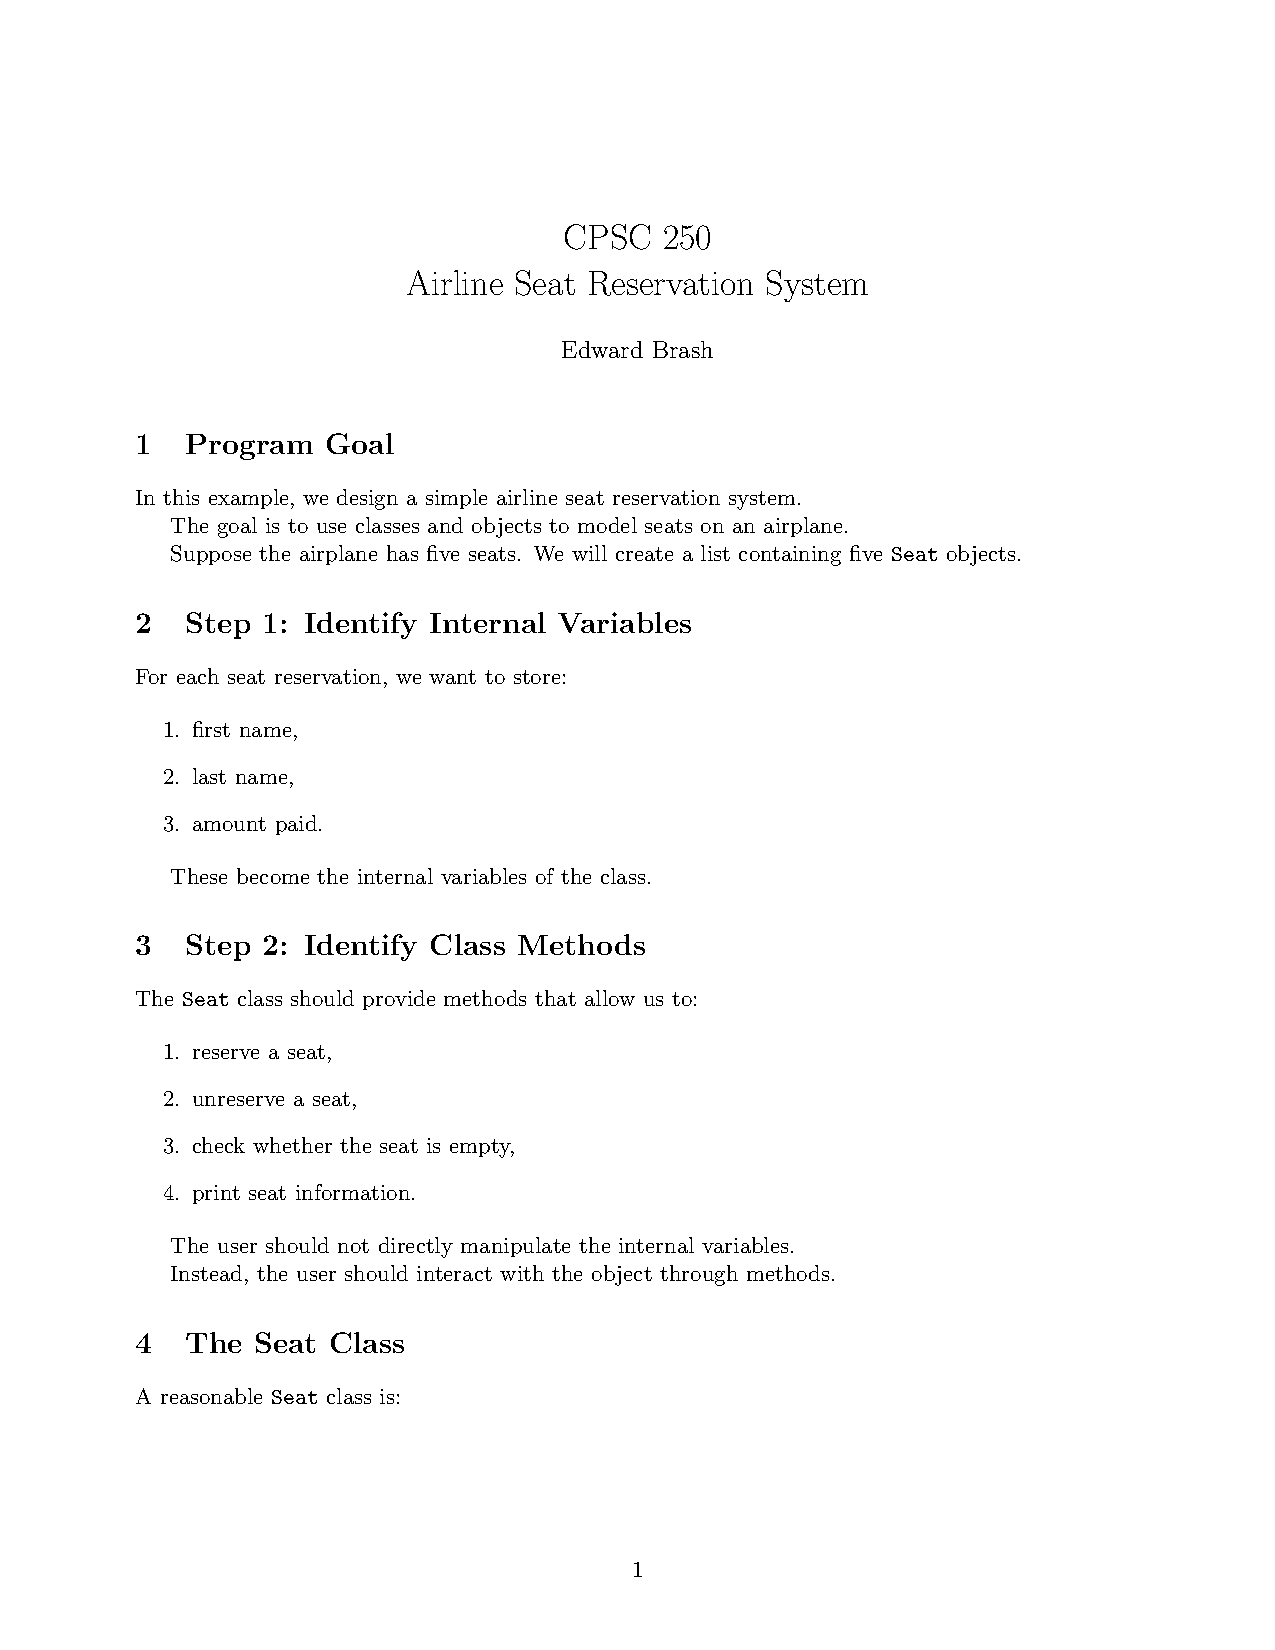
\includepdf[
    pages=-,
    addtotoc={1,subsection,2,{Airline Reservation System},week2h}
]{Week2_Lectures/week2h_airline_reservation_system.pdf}

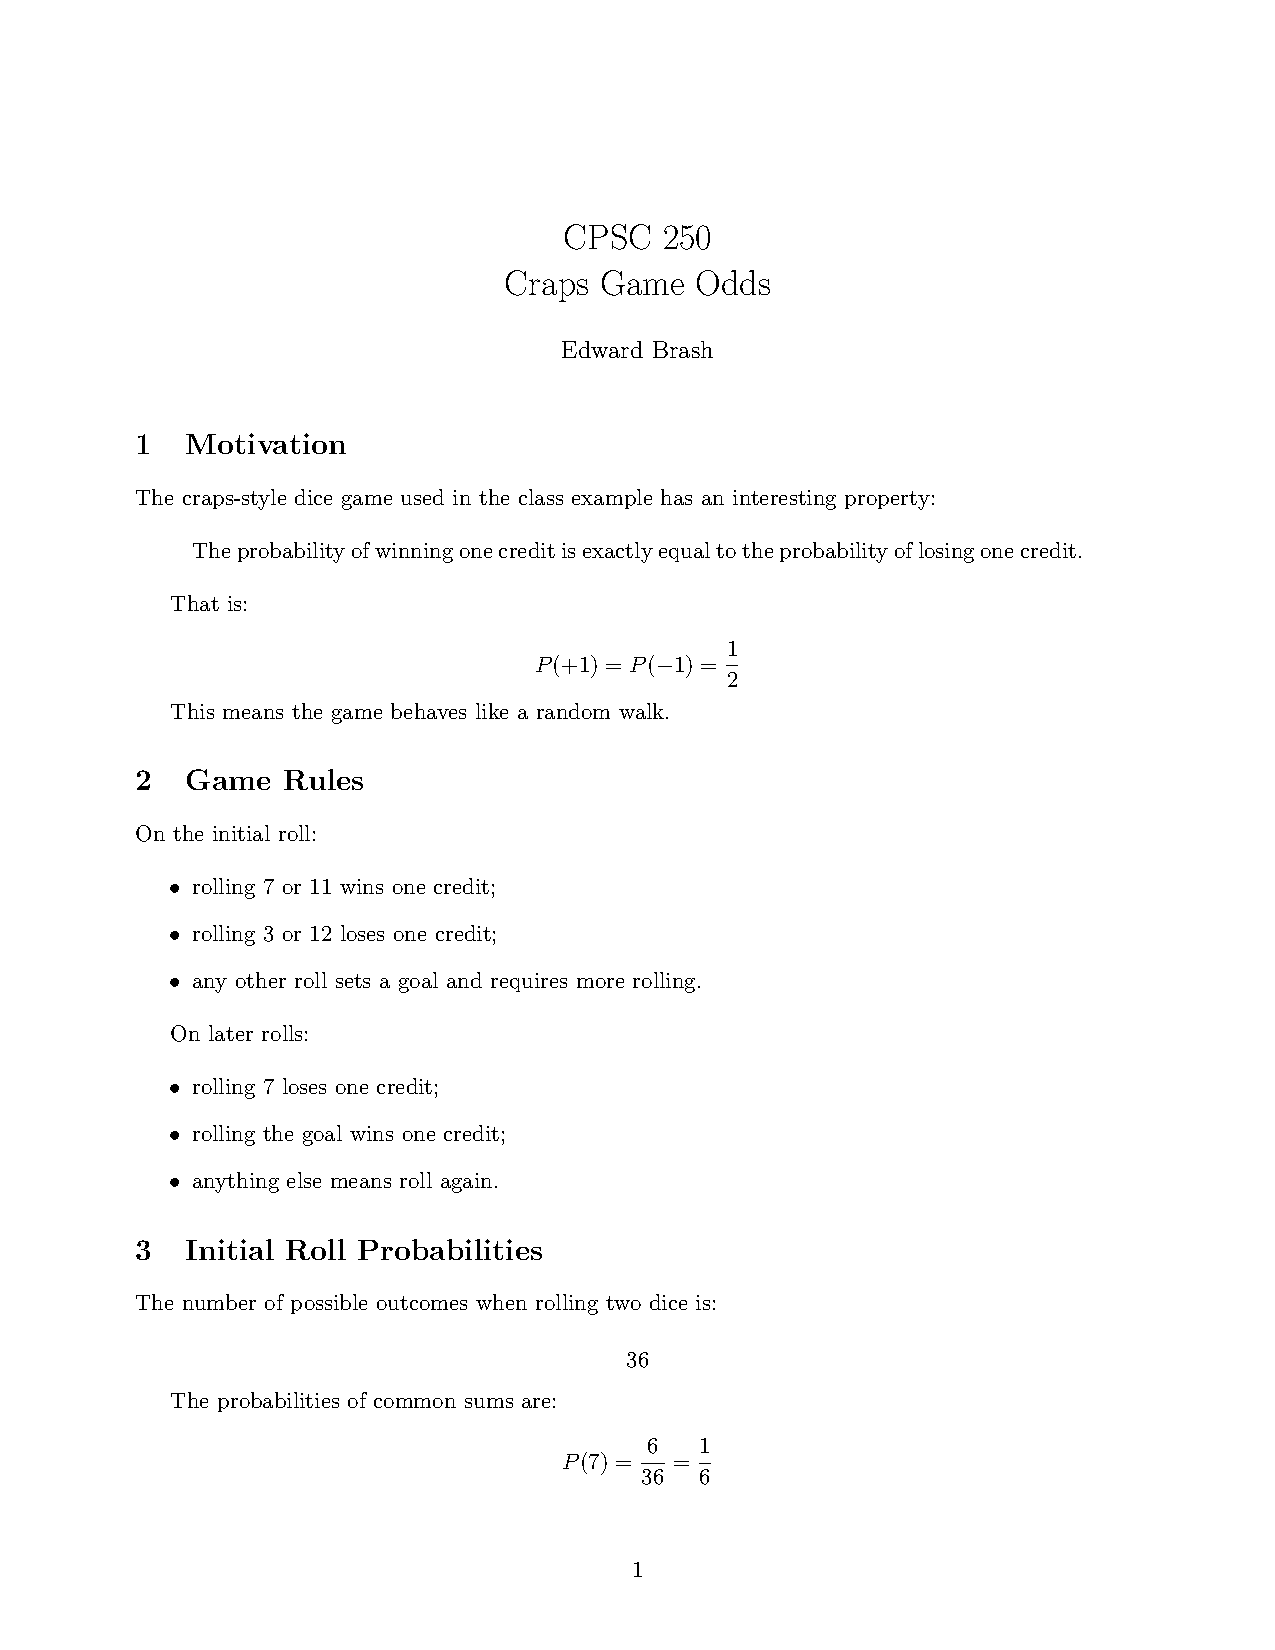
\includepdf[
    pages=-,
    addtotoc={1,subsection,2,{Craps Game Odds},week2i}
]{Week2_Lectures/week2i_craps_game_odds.pdf}

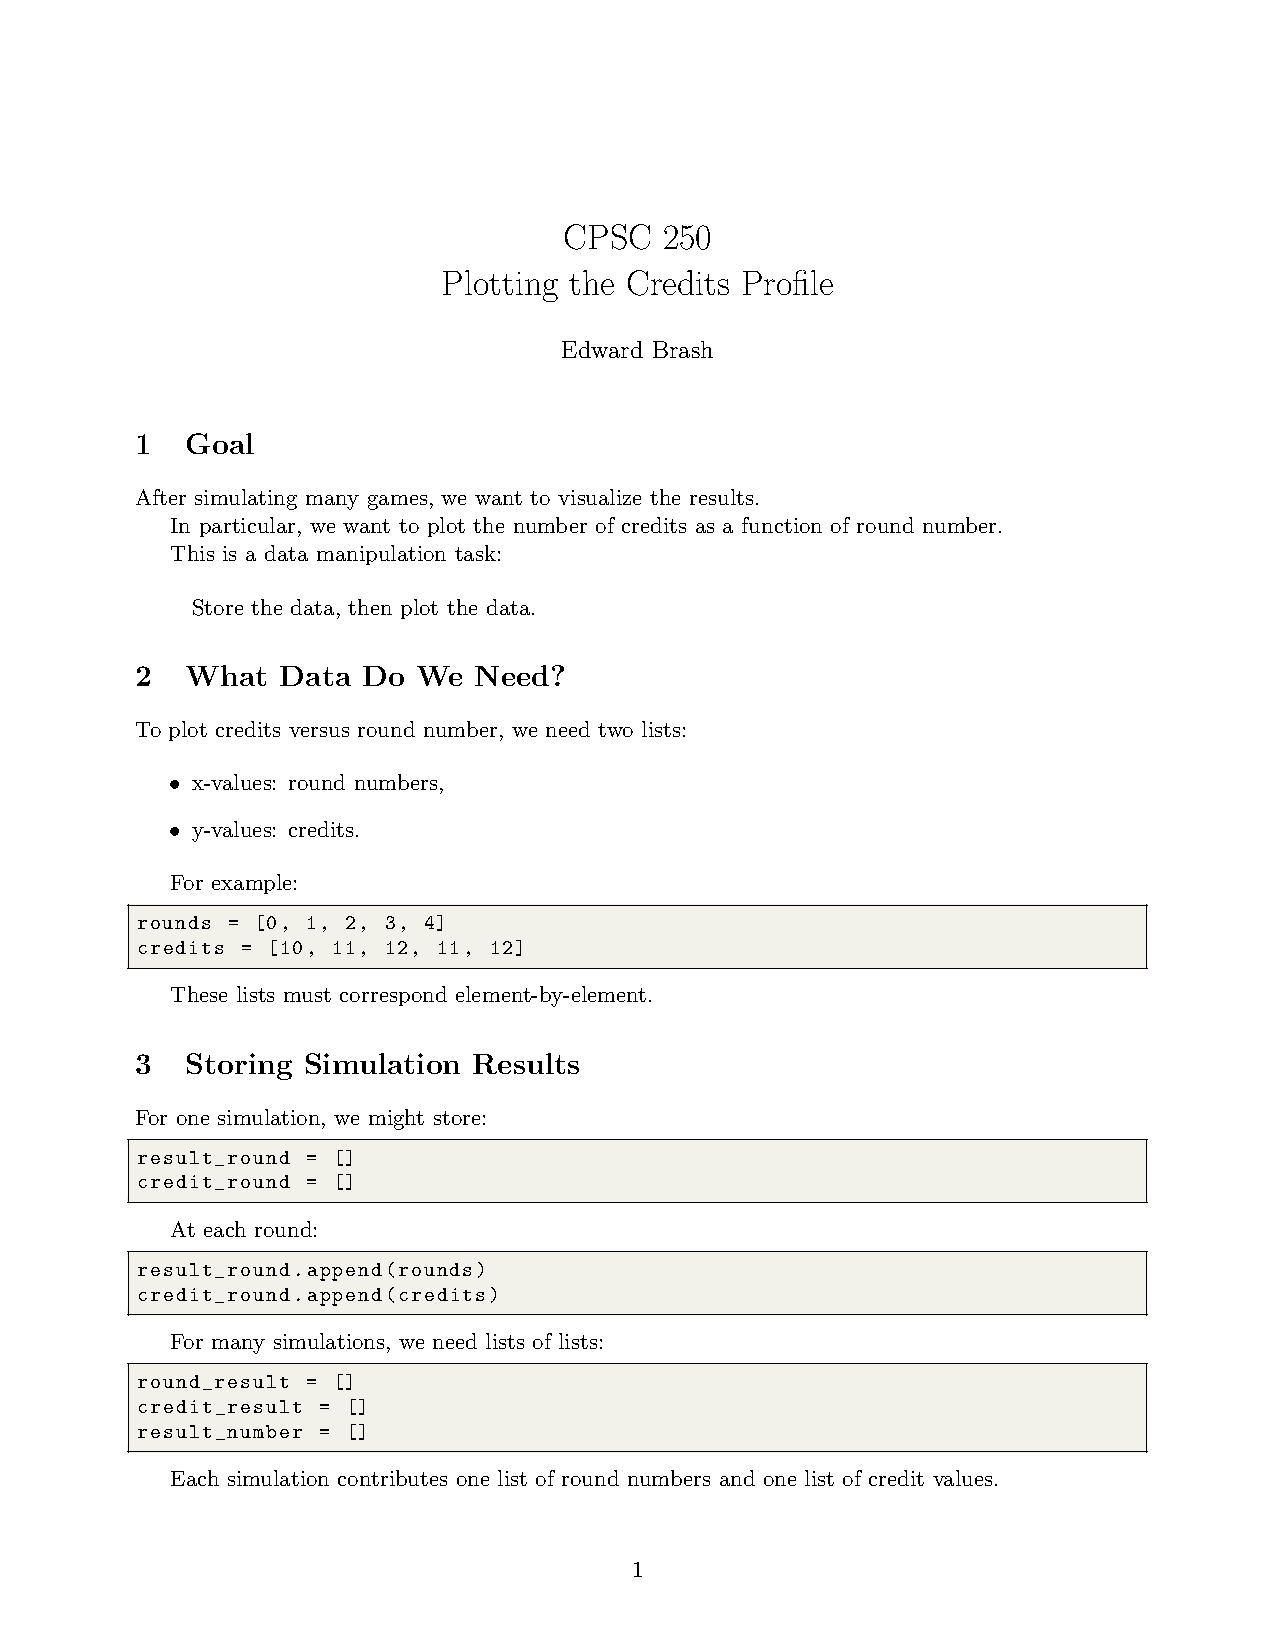
\includepdf[
    pages=-,
    addtotoc={1,subsection,2,{Plotting Credits},week2j}
]{Week2_Lectures/week2j_plotting_credits.pdf}

% ============================================================
% Week 3
% ============================================================

\clearpage
\section*{Week 3: Inheritance, Recursion, Algorithms, and Testing}
\addcontentsline{toc}{section}{Week 3: Inheritance, Recursion, Algorithms, and Testing}

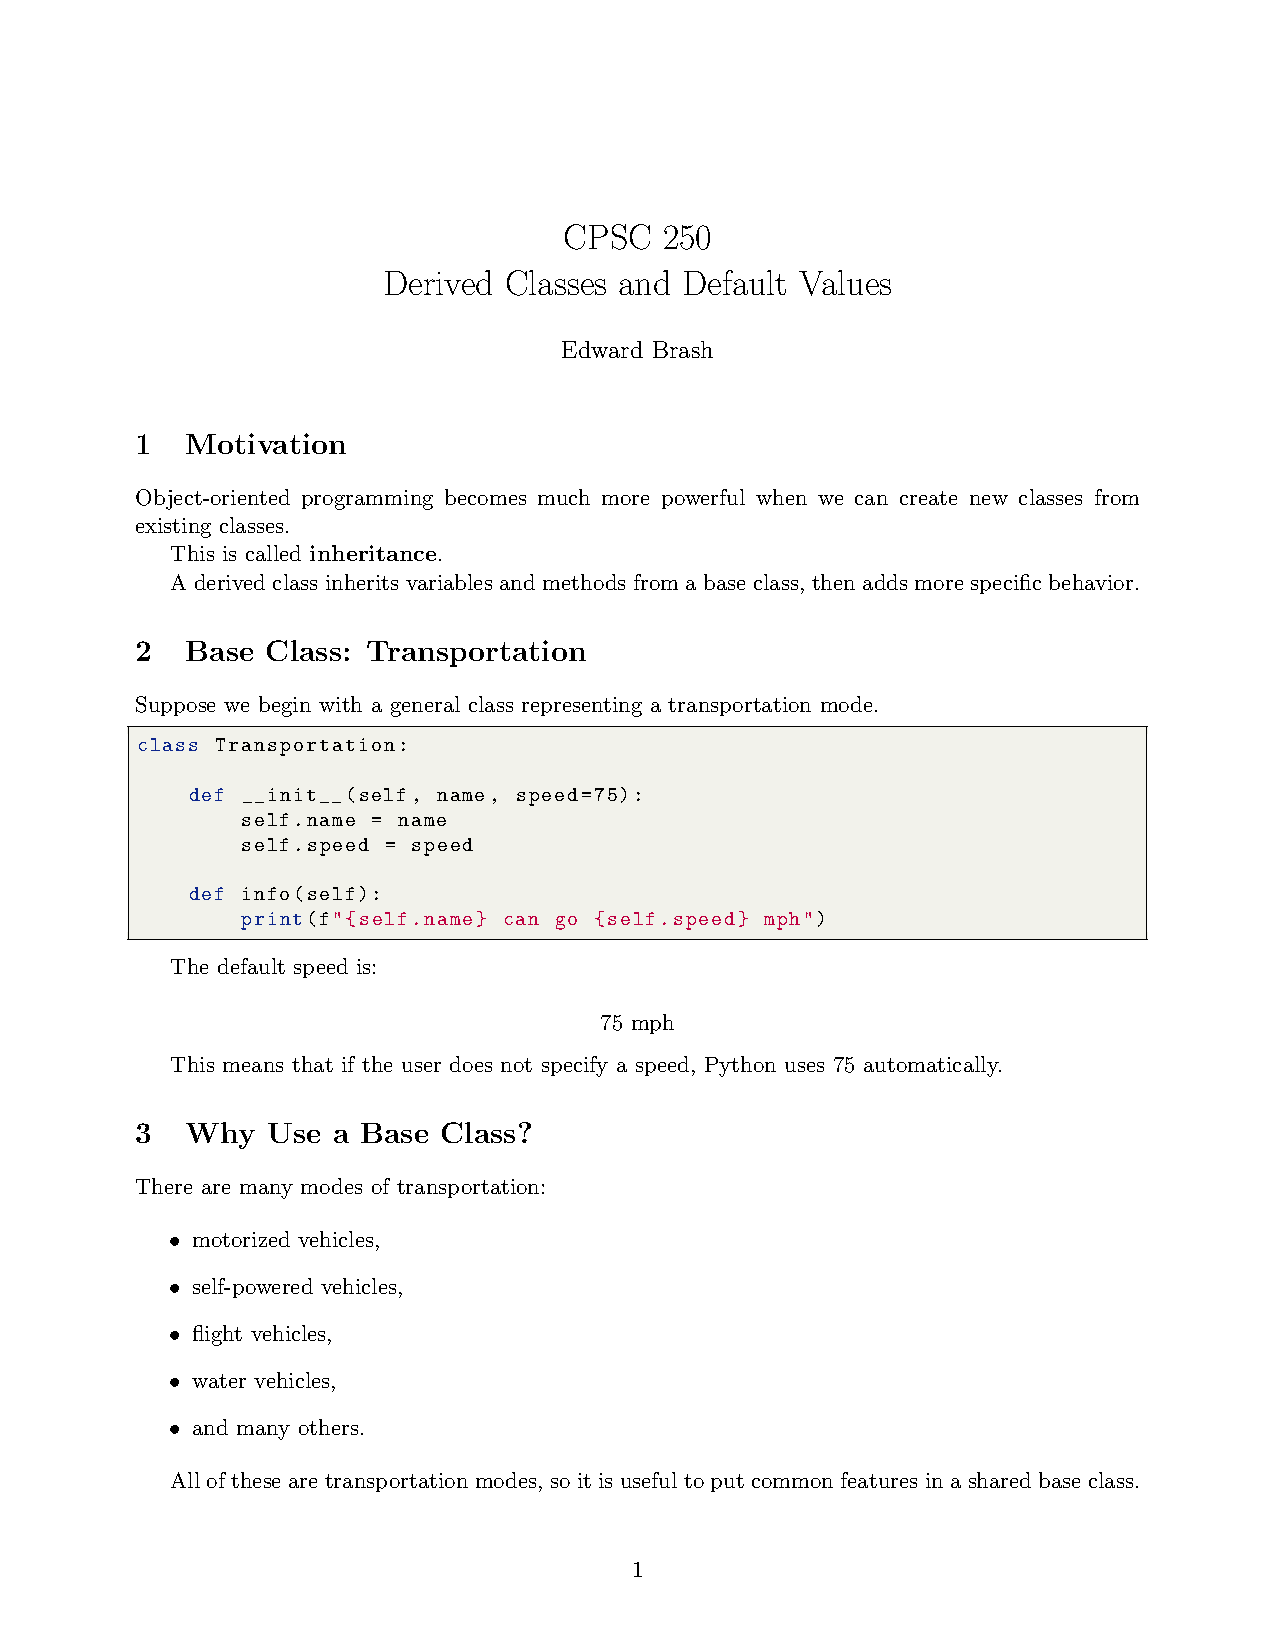
\includepdf[
    pages=-,
    addtotoc={1,subsection,2,{Derived Classes},week3a}
]{Week3_Lectures/week3a_derived_classes.pdf}

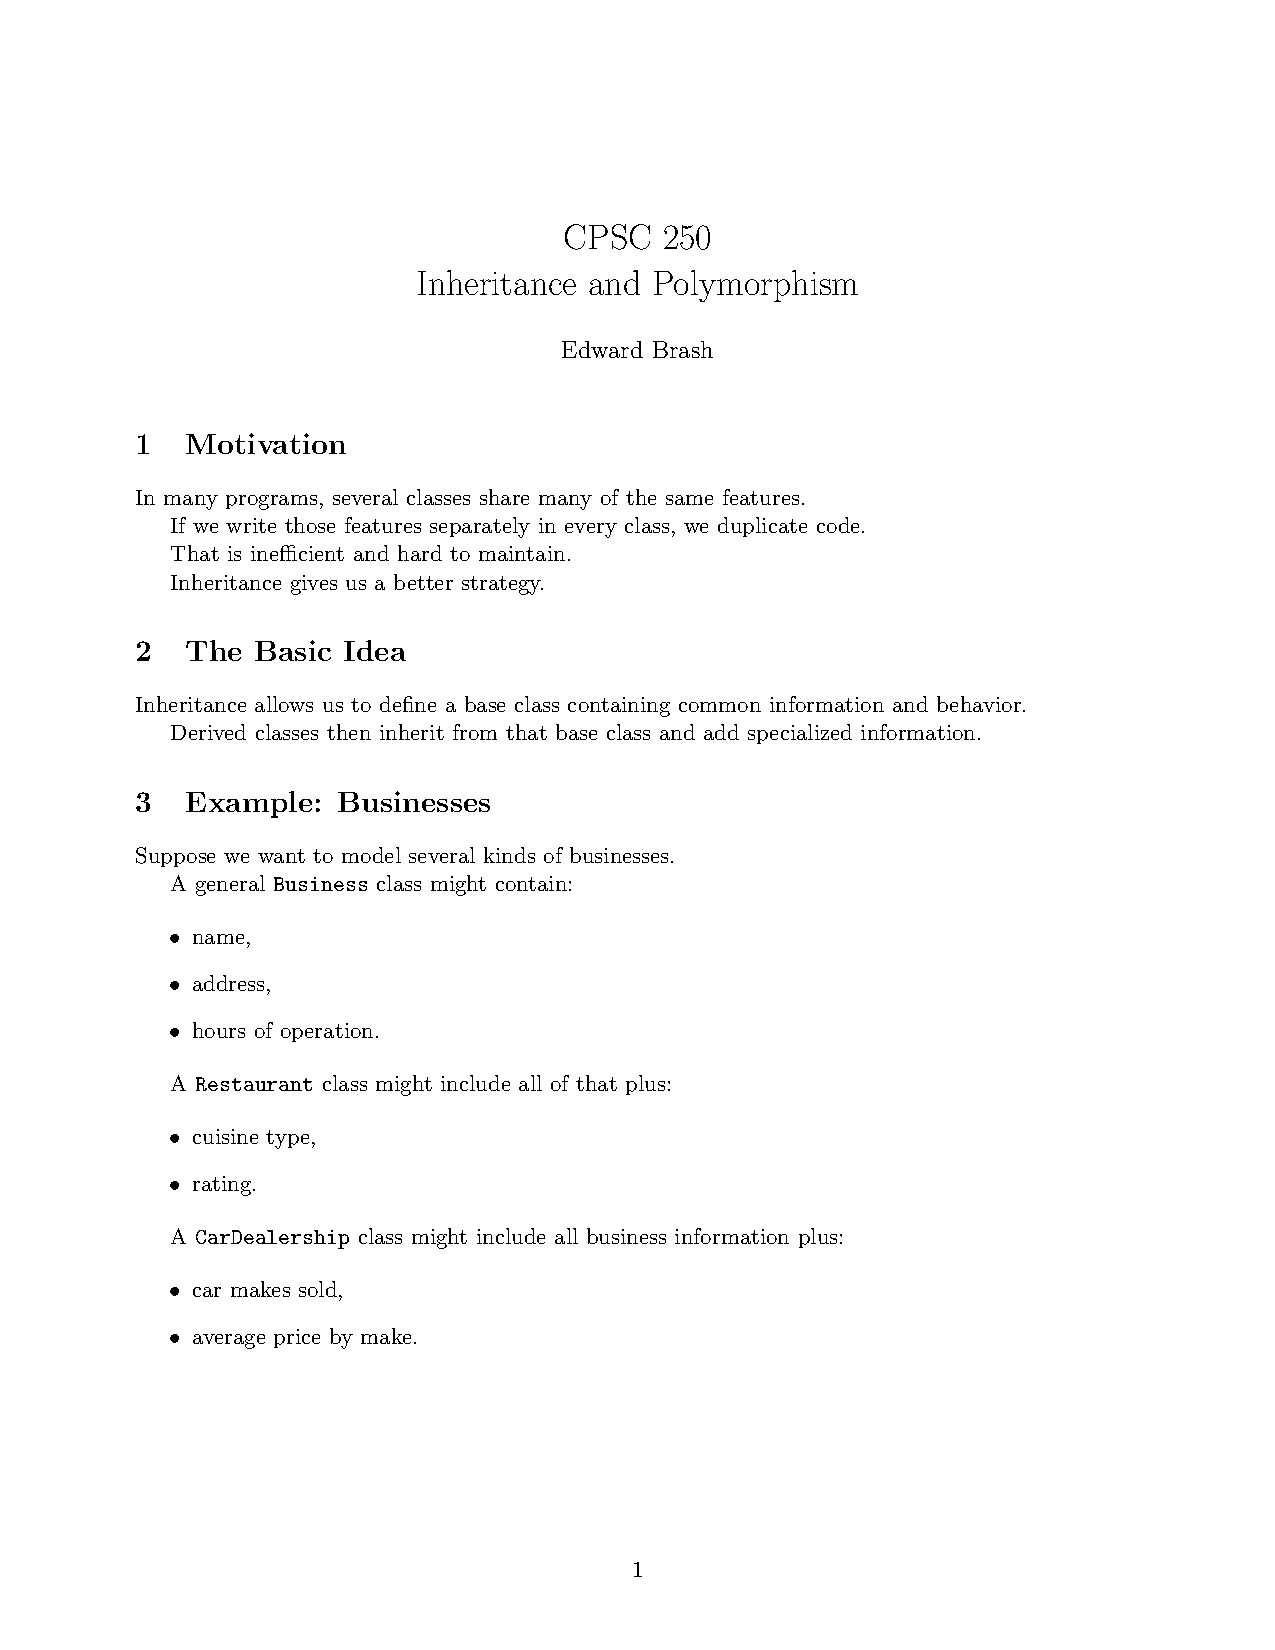
\includepdf[
    pages=-,
    addtotoc={1,subsection,2,{Inheritance and Polymorphism},week3b}
]{Week3_Lectures/week3b_inheritance_polymorphism.pdf}

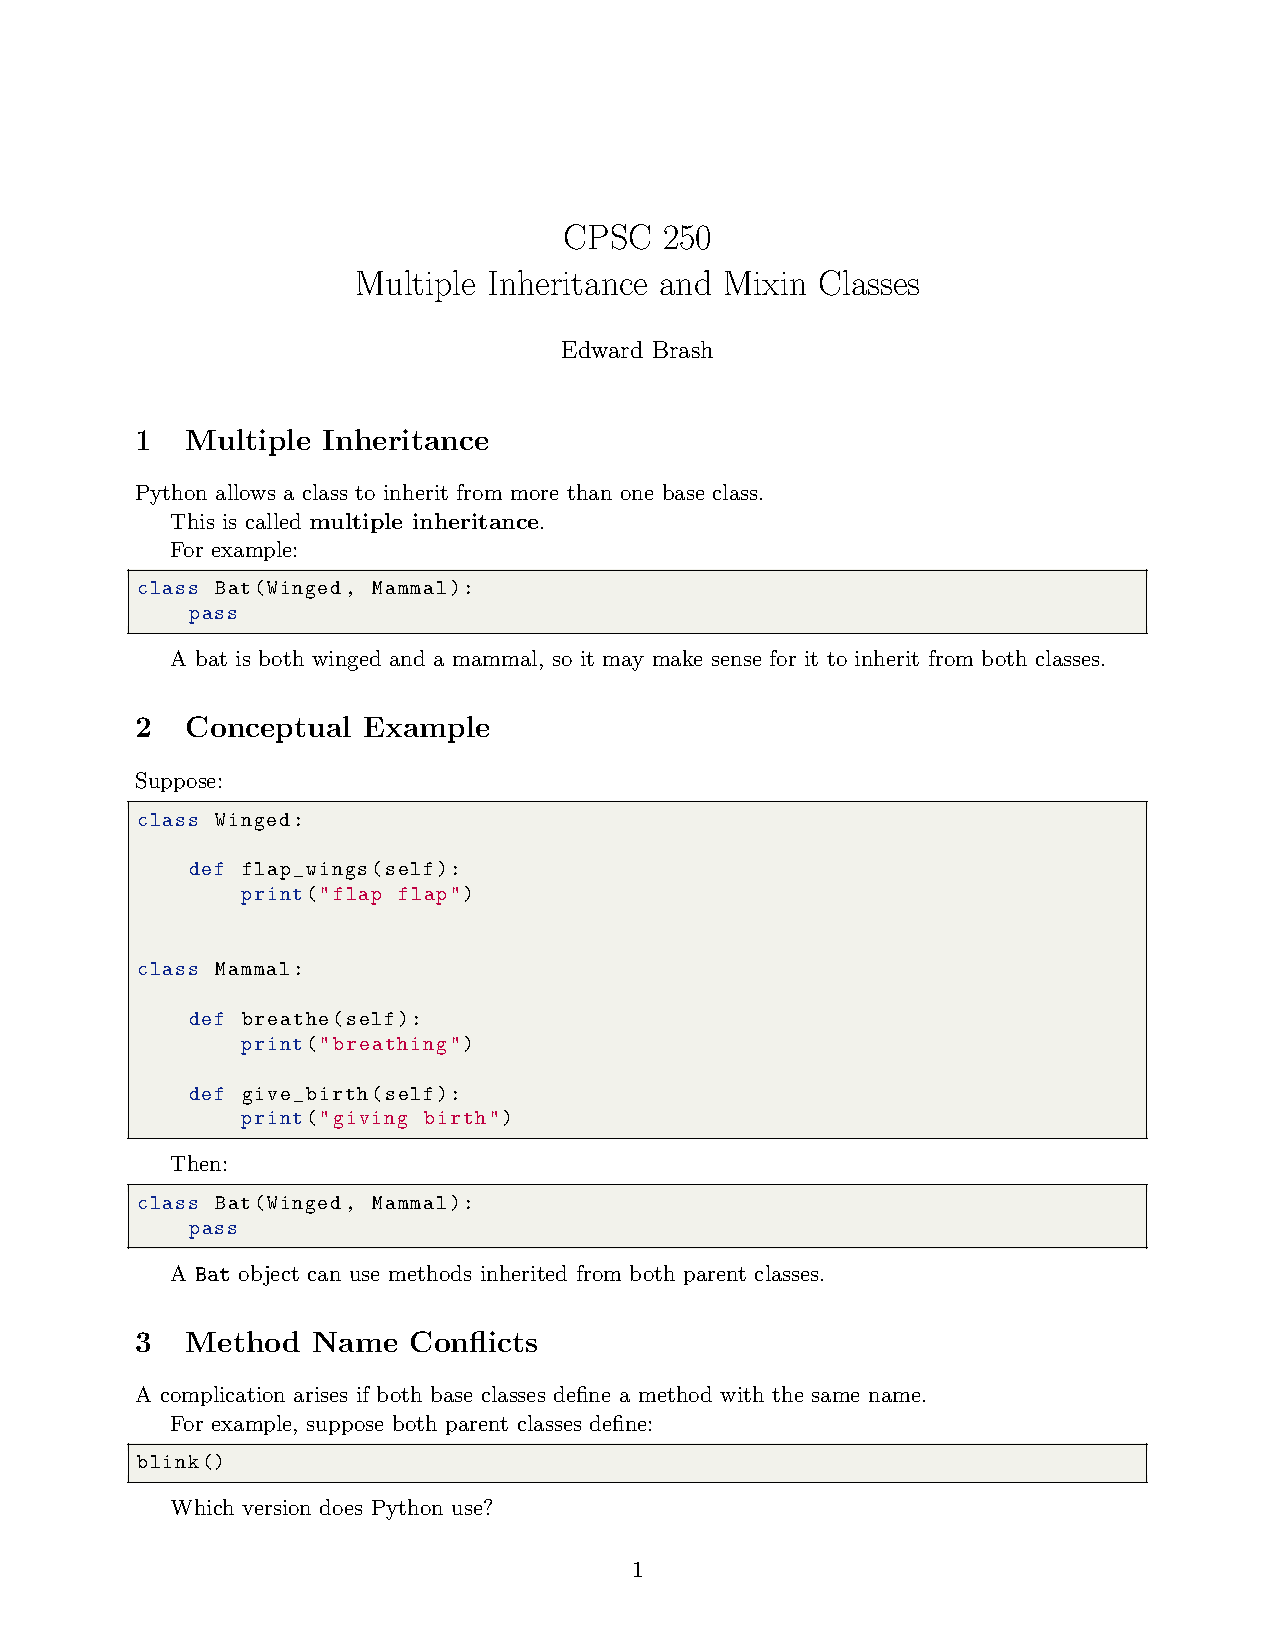
\includepdf[
    pages=-,
    addtotoc={1,subsection,2,{Multiple Inheritance and Mixins},week3c}
]{Week3_Lectures/week3c_multiple_inheritance_mixins.pdf}

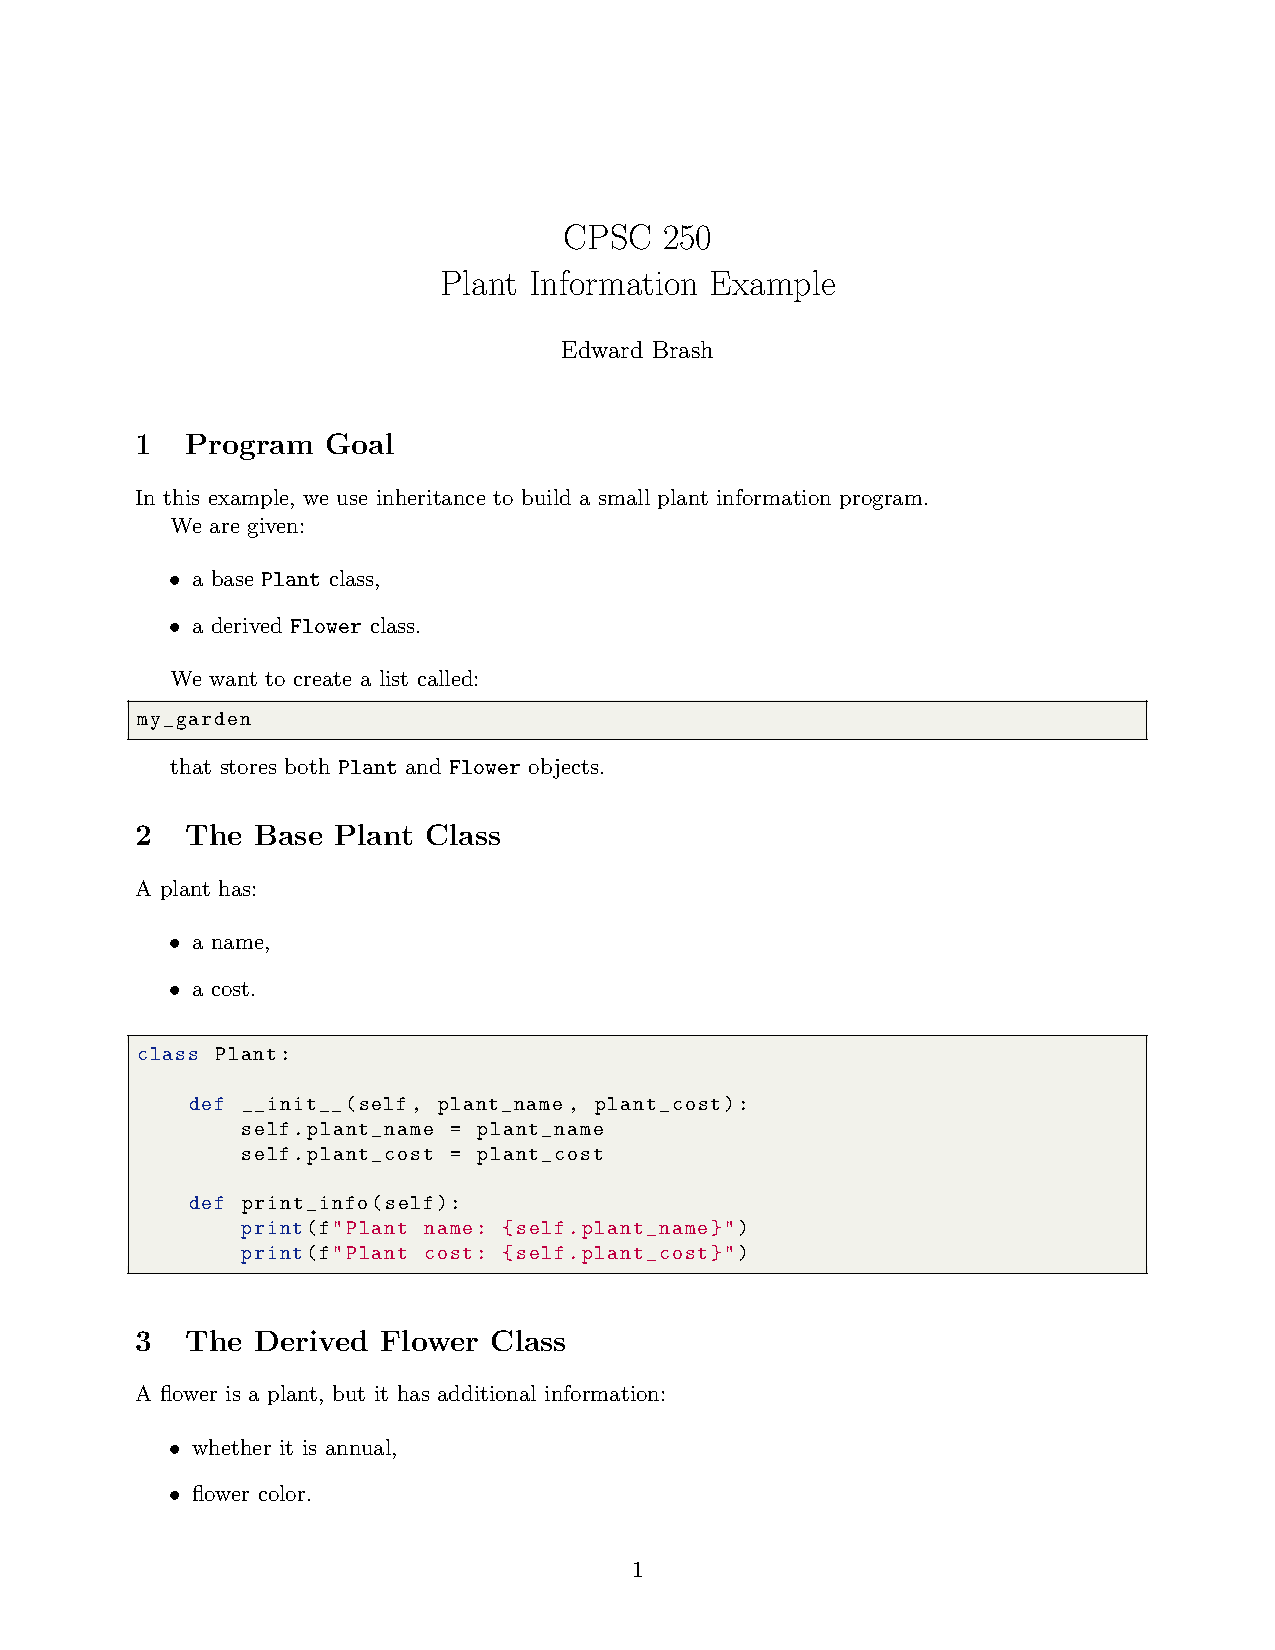
\includepdf[
    pages=-,
    addtotoc={1,subsection,2,{Plant Information Example},week3d}
]{Week3_Lectures/week3d_plant_information_example.pdf}

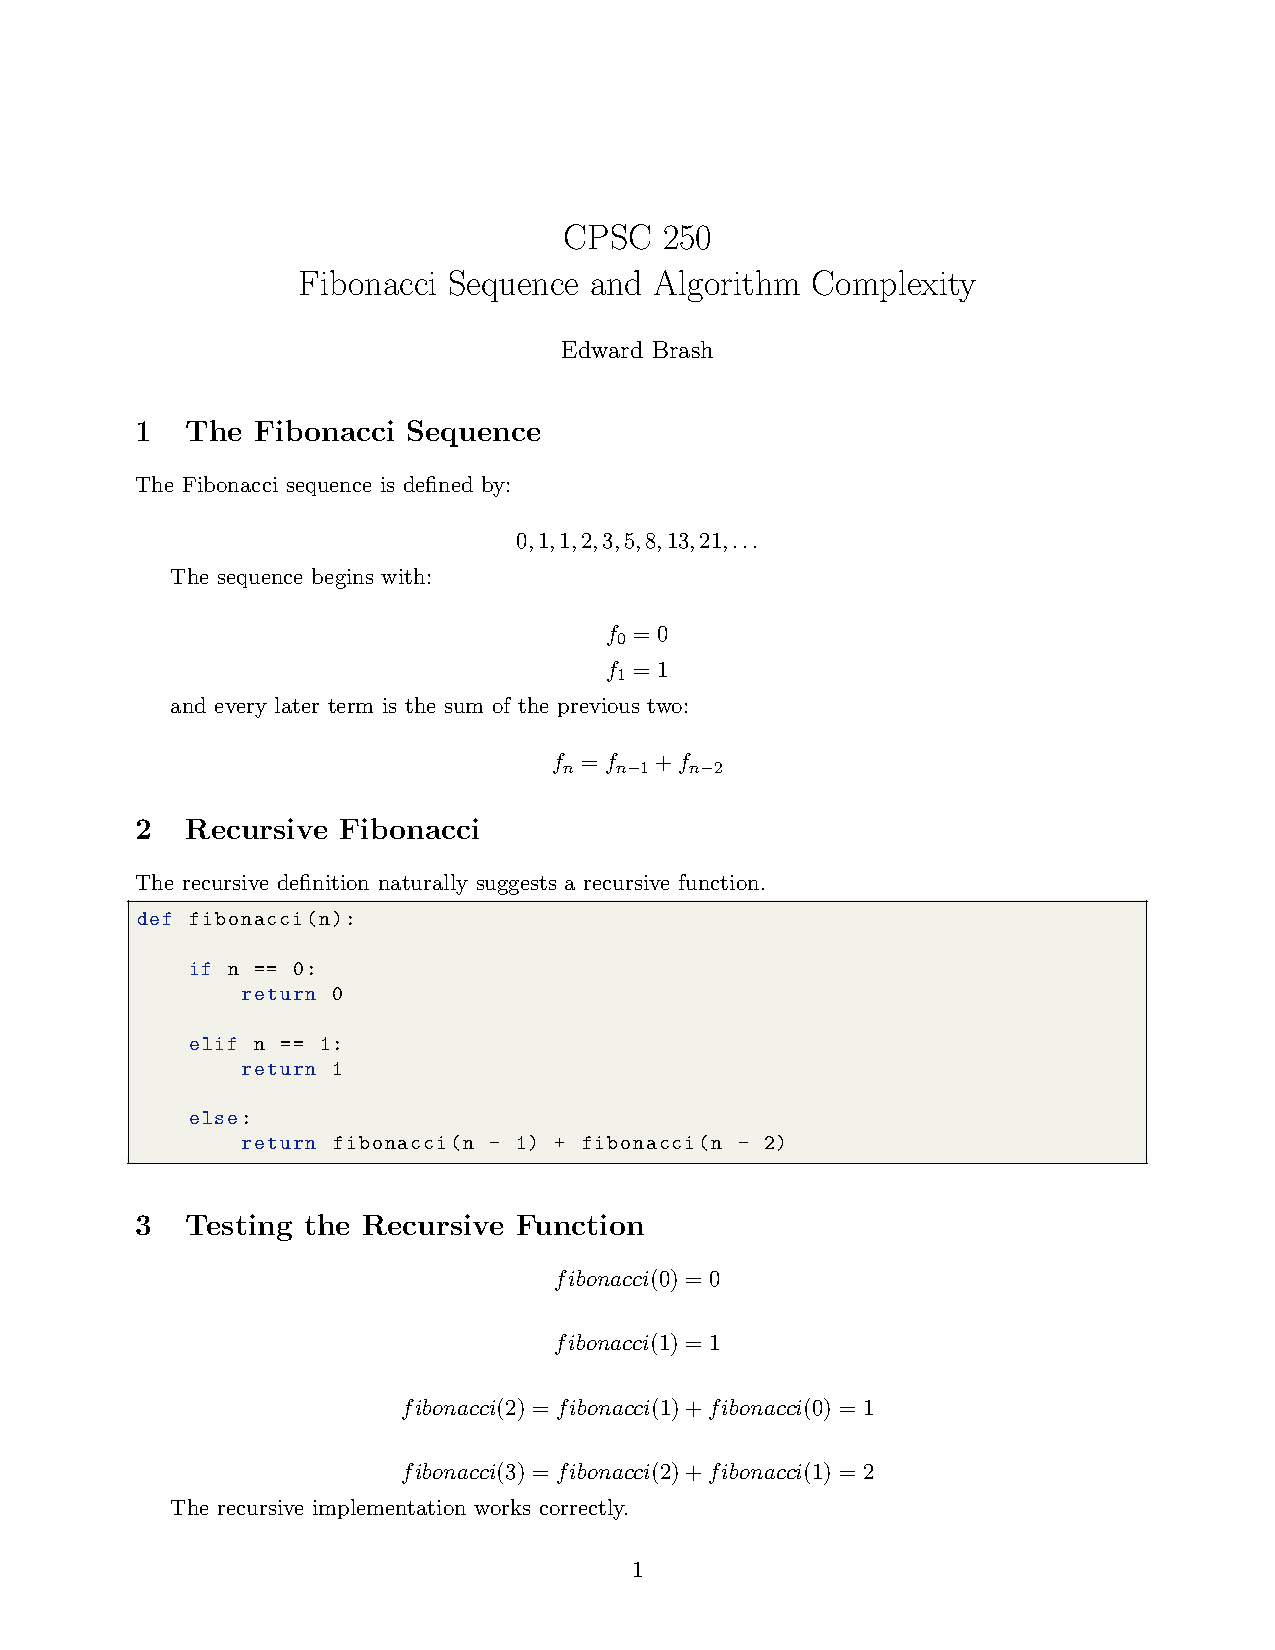
\includepdf[
    pages=-,
    addtotoc={1,subsection,2,{Fibonacci},week3e}
]{Week3_Lectures/week3e_fibonacci.pdf}

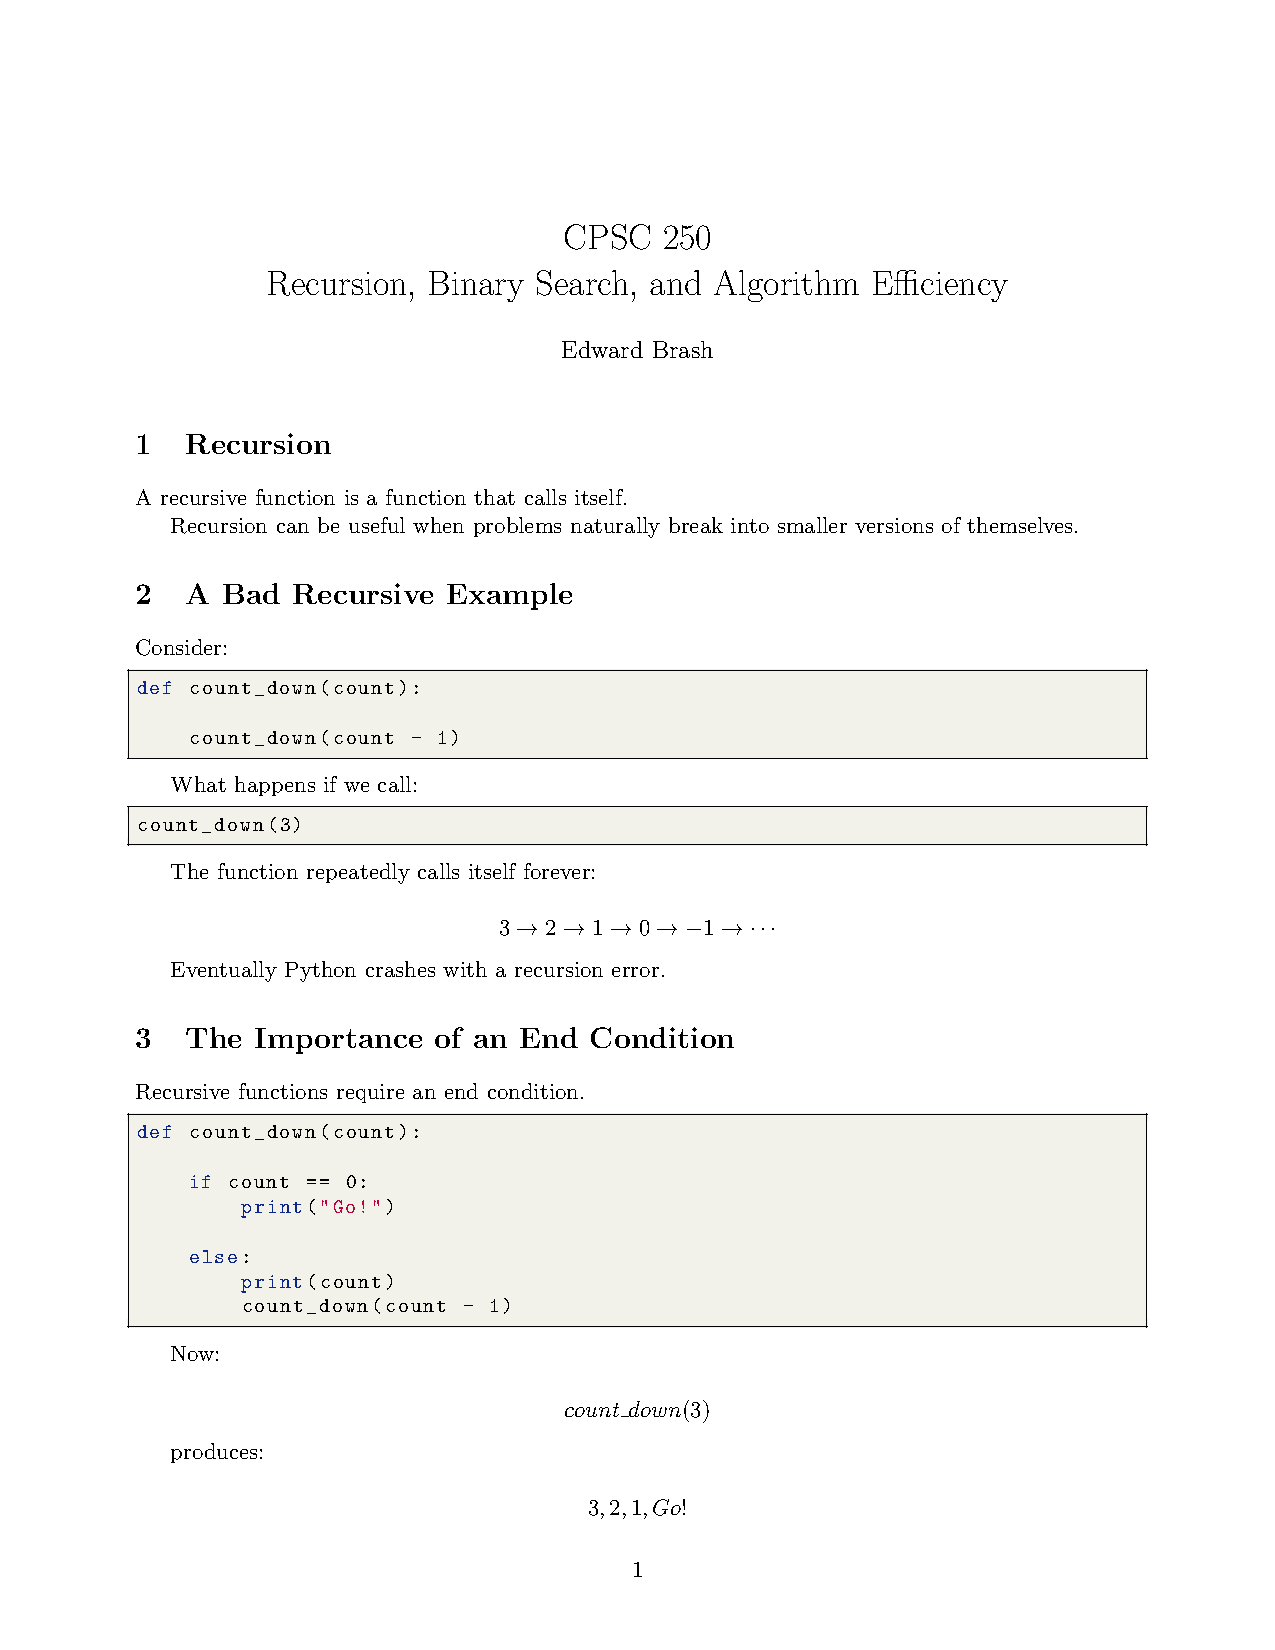
\includepdf[
    pages=-,
    addtotoc={1,subsection,2,{Complex Algorithms},week3f}
]{Week3_Lectures/week3f_complex_algorithms.pdf}

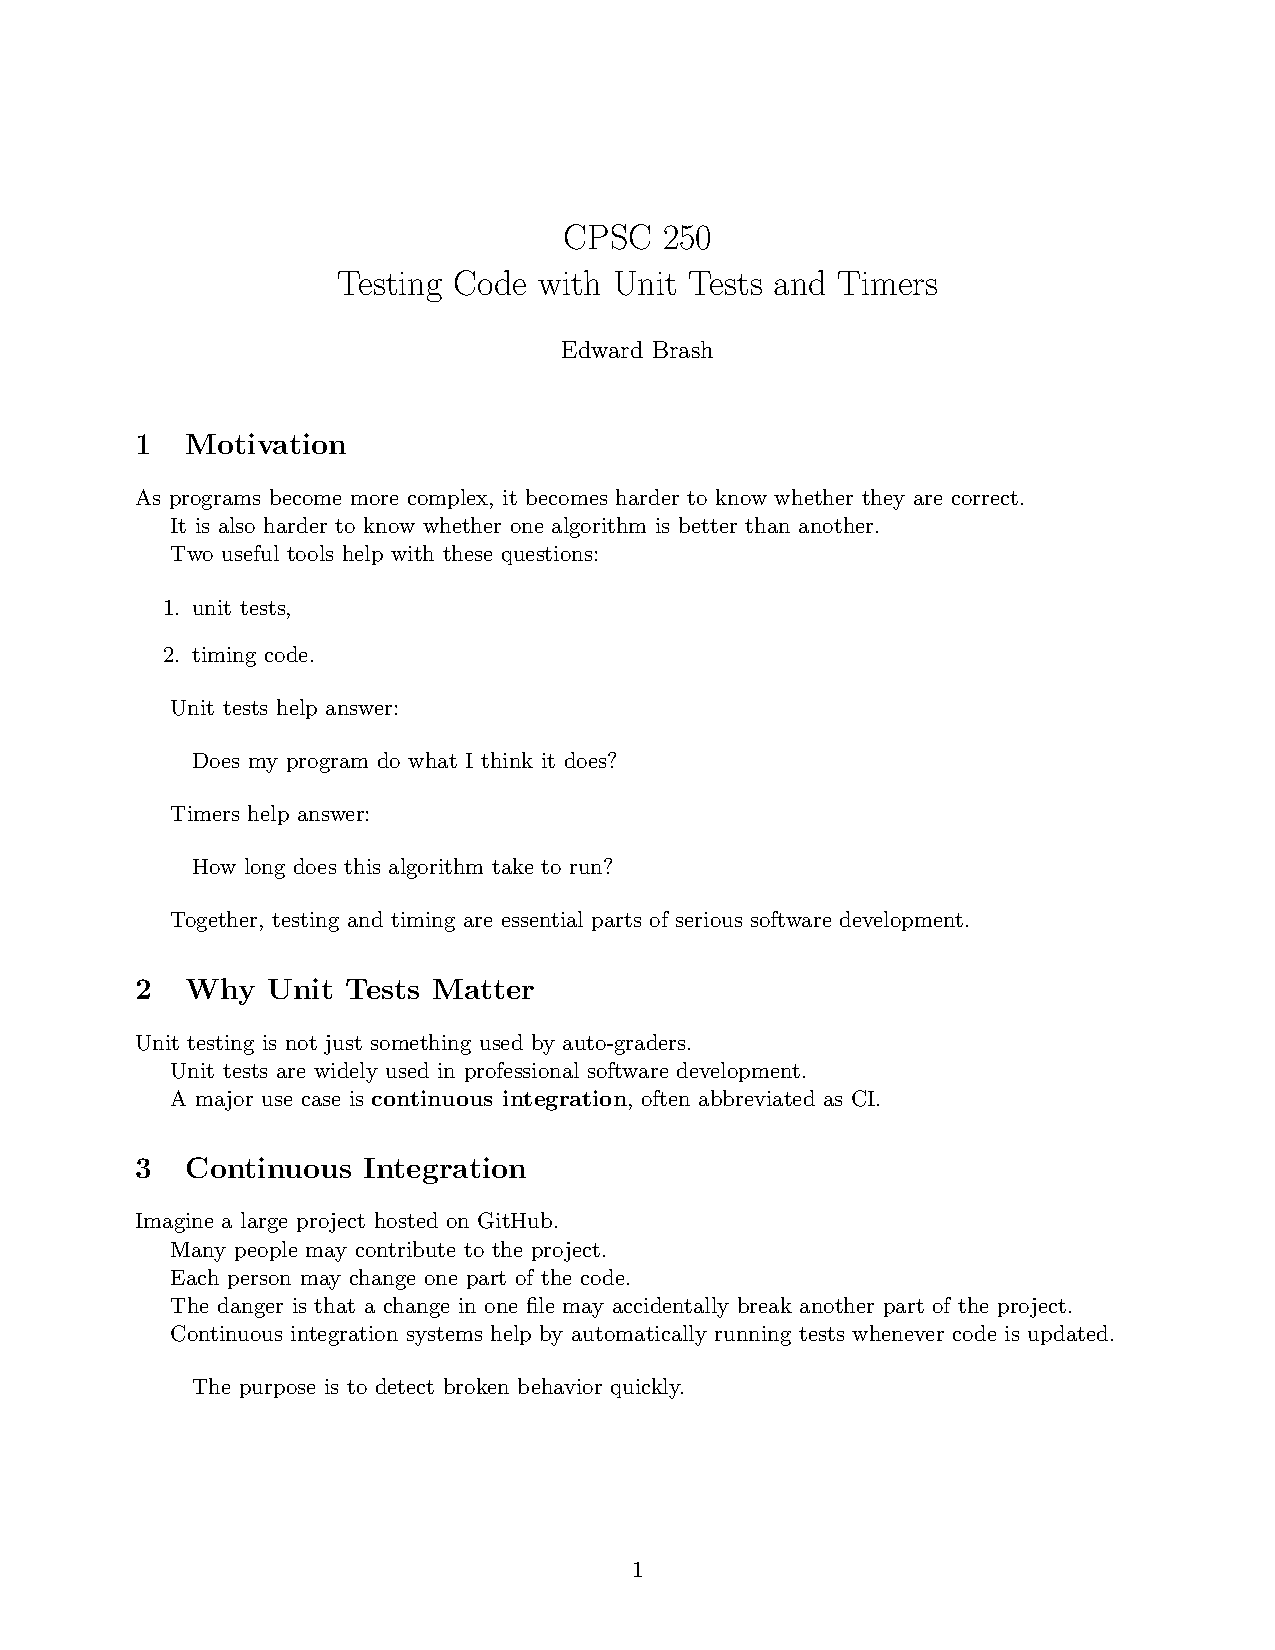
\includepdf[
    pages=-,
    addtotoc={1,subsection,2,{Unit Tests and Timers},week3g}
]{Week3_Lectures/week3g_unit_tests_and_timers.pdf}

% ============================================================
% Week 4
% ============================================================

\clearpage
\section*{Week 4: Plotting, Regression, and Data Analysis}
\addcontentsline{toc}{section}{Week 4: Plotting, Regression, and Data Analysis}

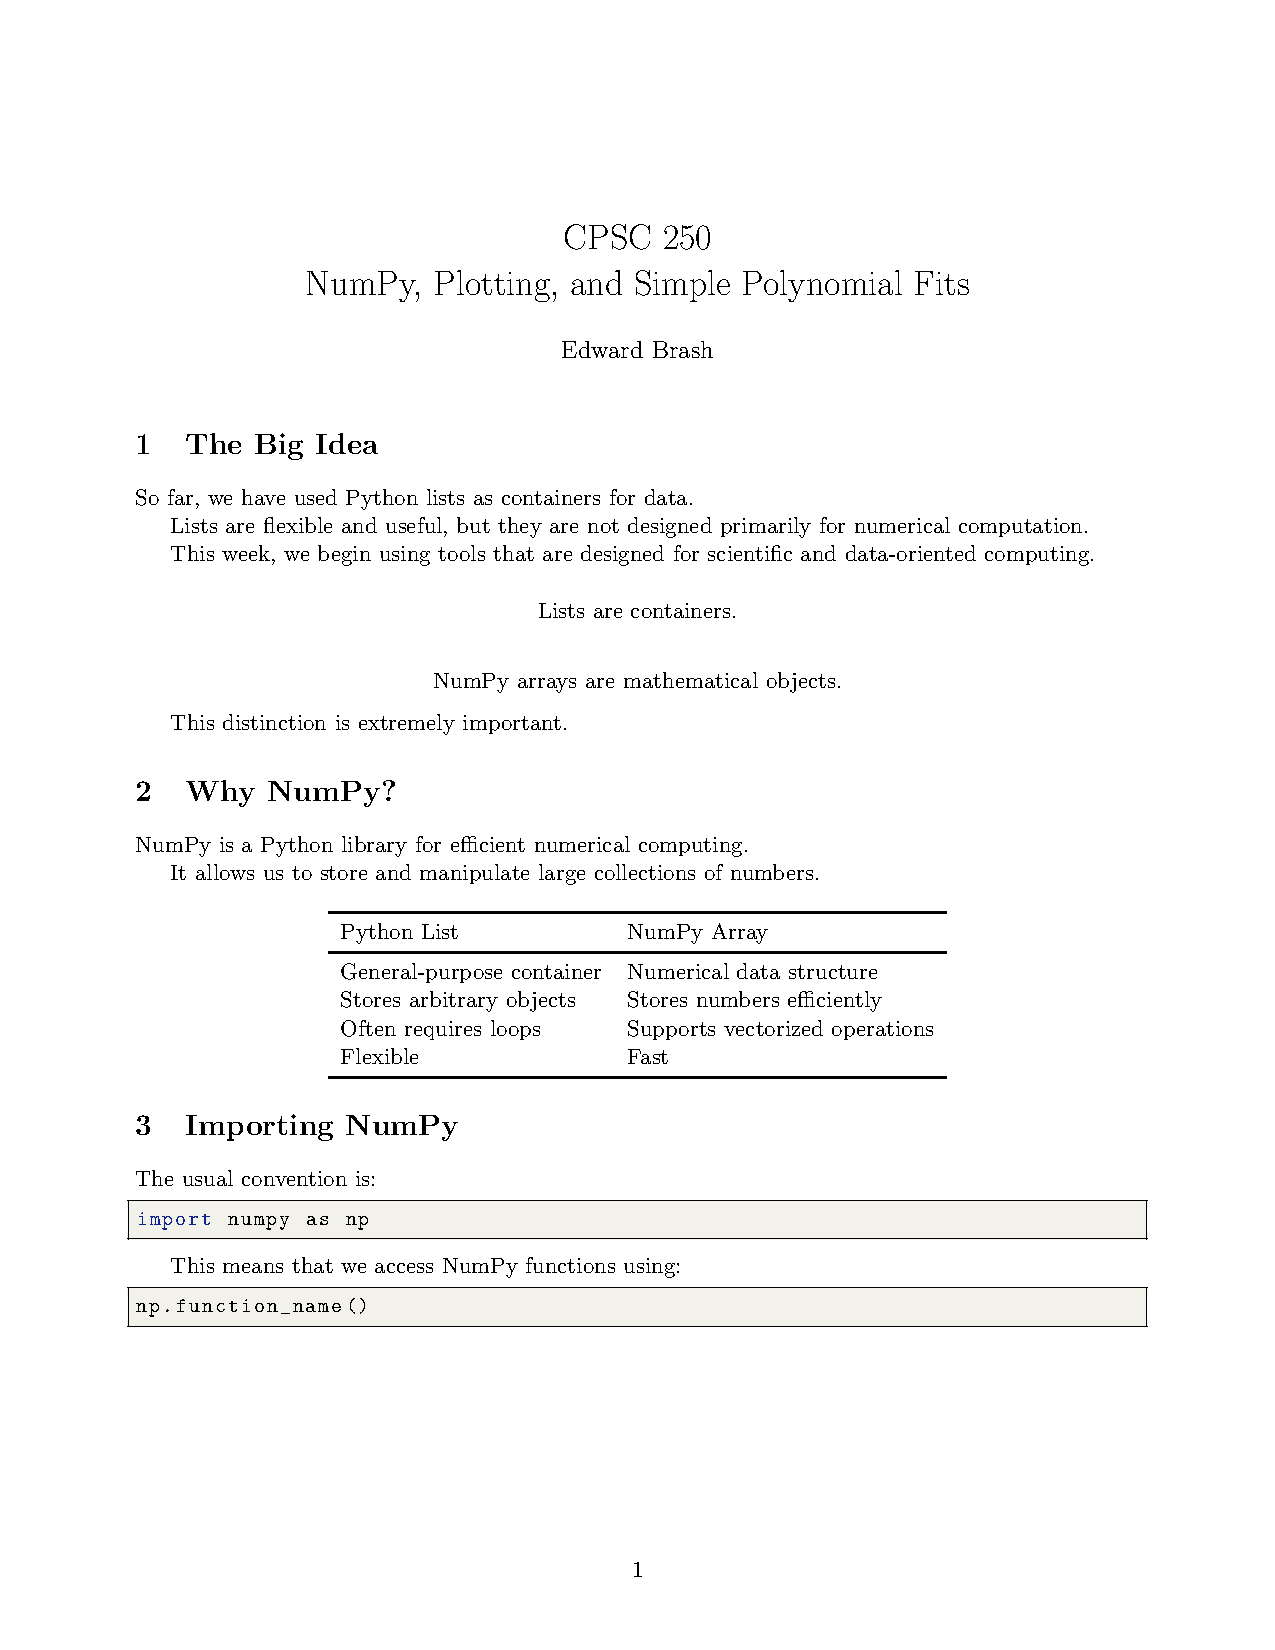
\includepdf[
    pages=-,
    addtotoc={1,subsection,2,{Fitting with Numpy.polyfit},week4a}
]{Week4_Lectures/week4a_numpy_polyfit.pdf}

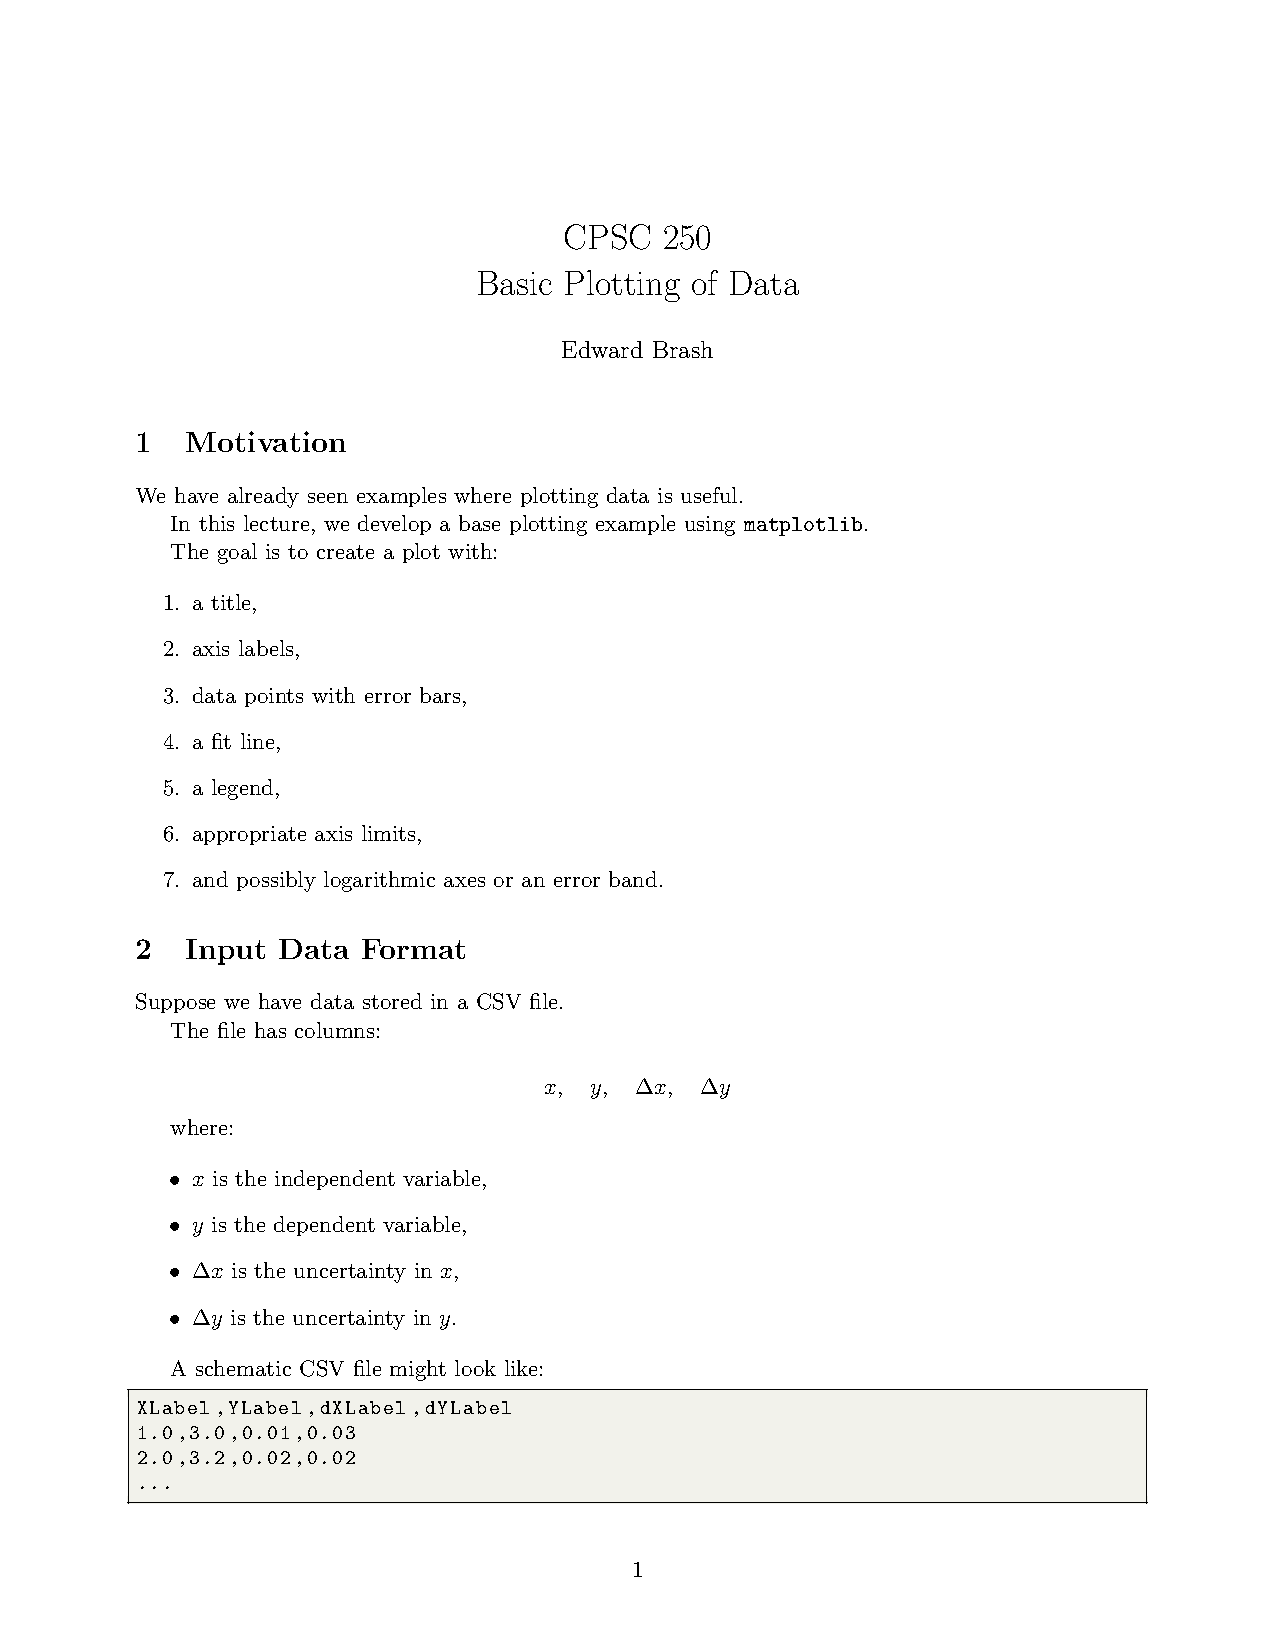
\includepdf[
    pages=-,
    addtotoc={1,subsection,2,{Basic Plotting of Data},week4b}
]{Week4_Lectures/week4b_basic_plotting_data.pdf}

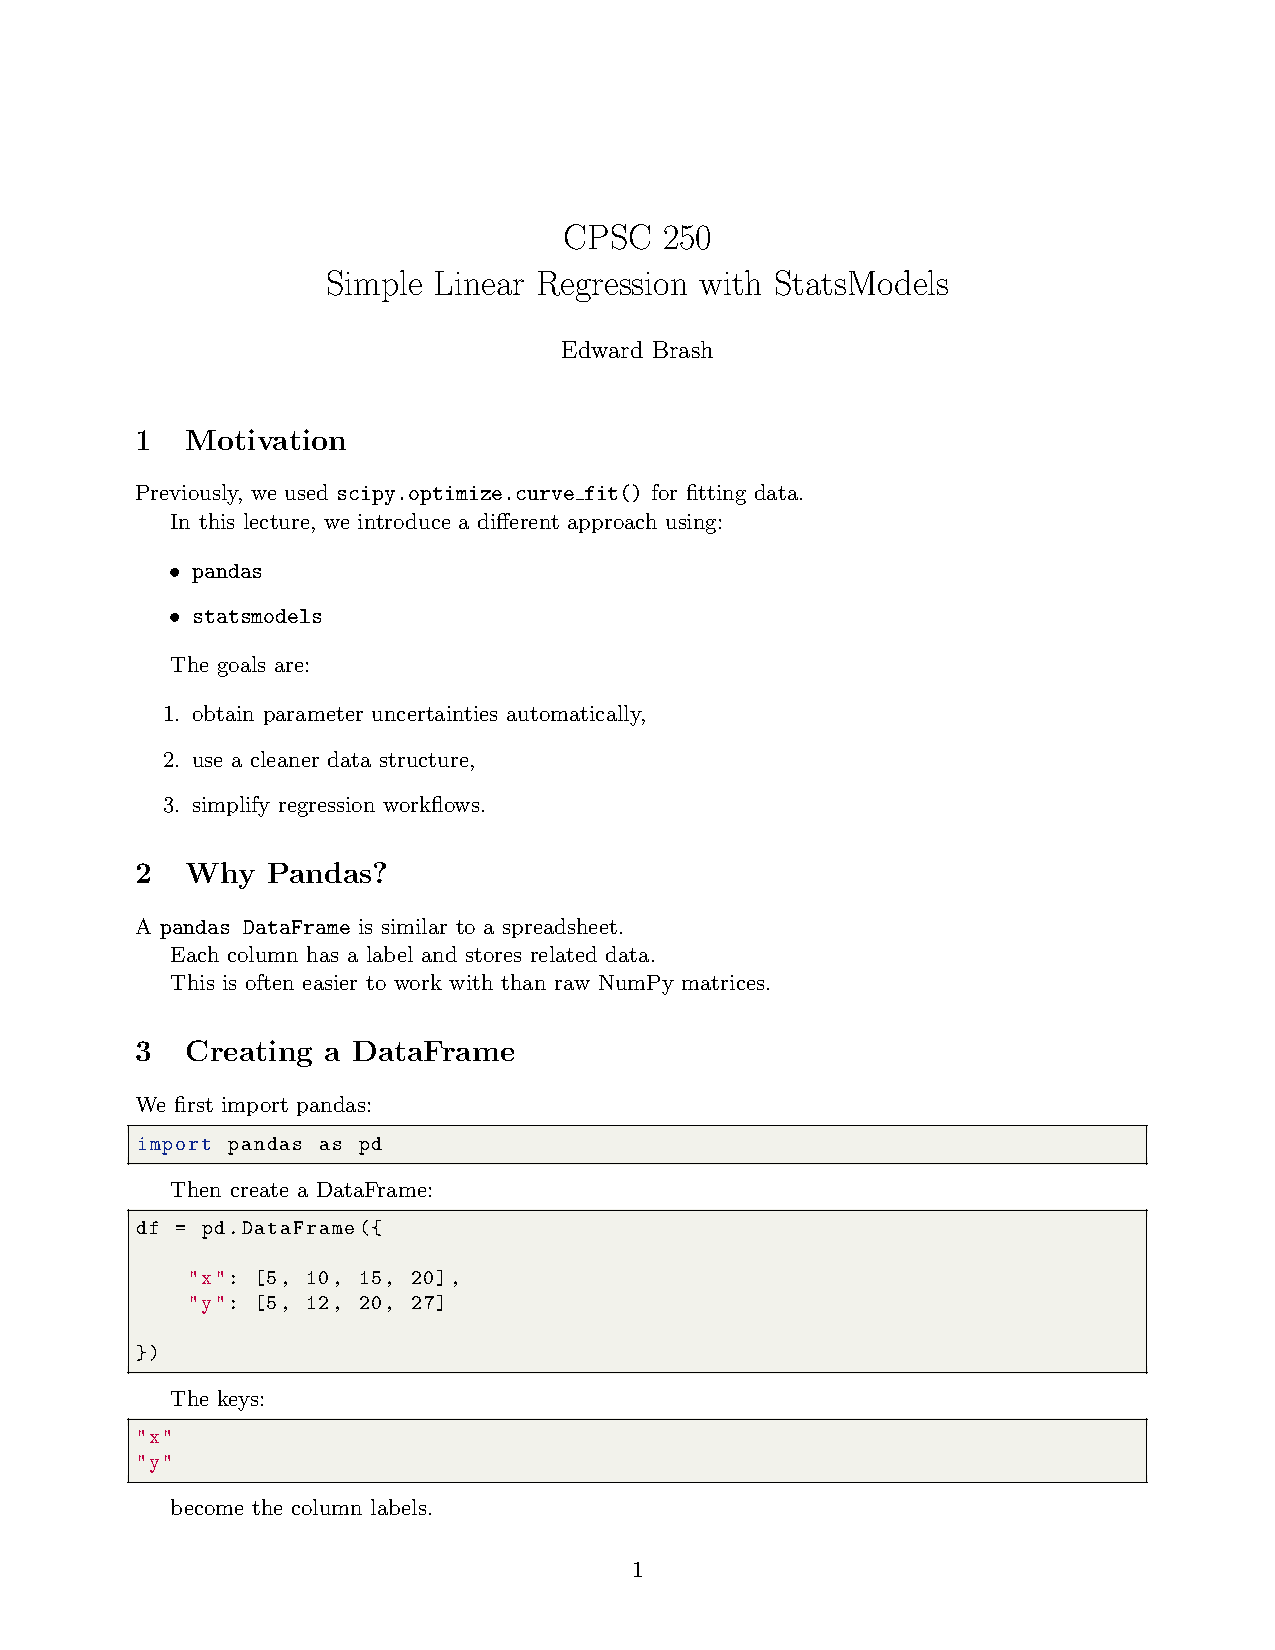
\includepdf[
    pages=-,
    addtotoc={1,subsection,2,{StatsModels Linear Regression},week4c}
]{Week4_Lectures/week4c_statsmodels_linear_regression.pdf}

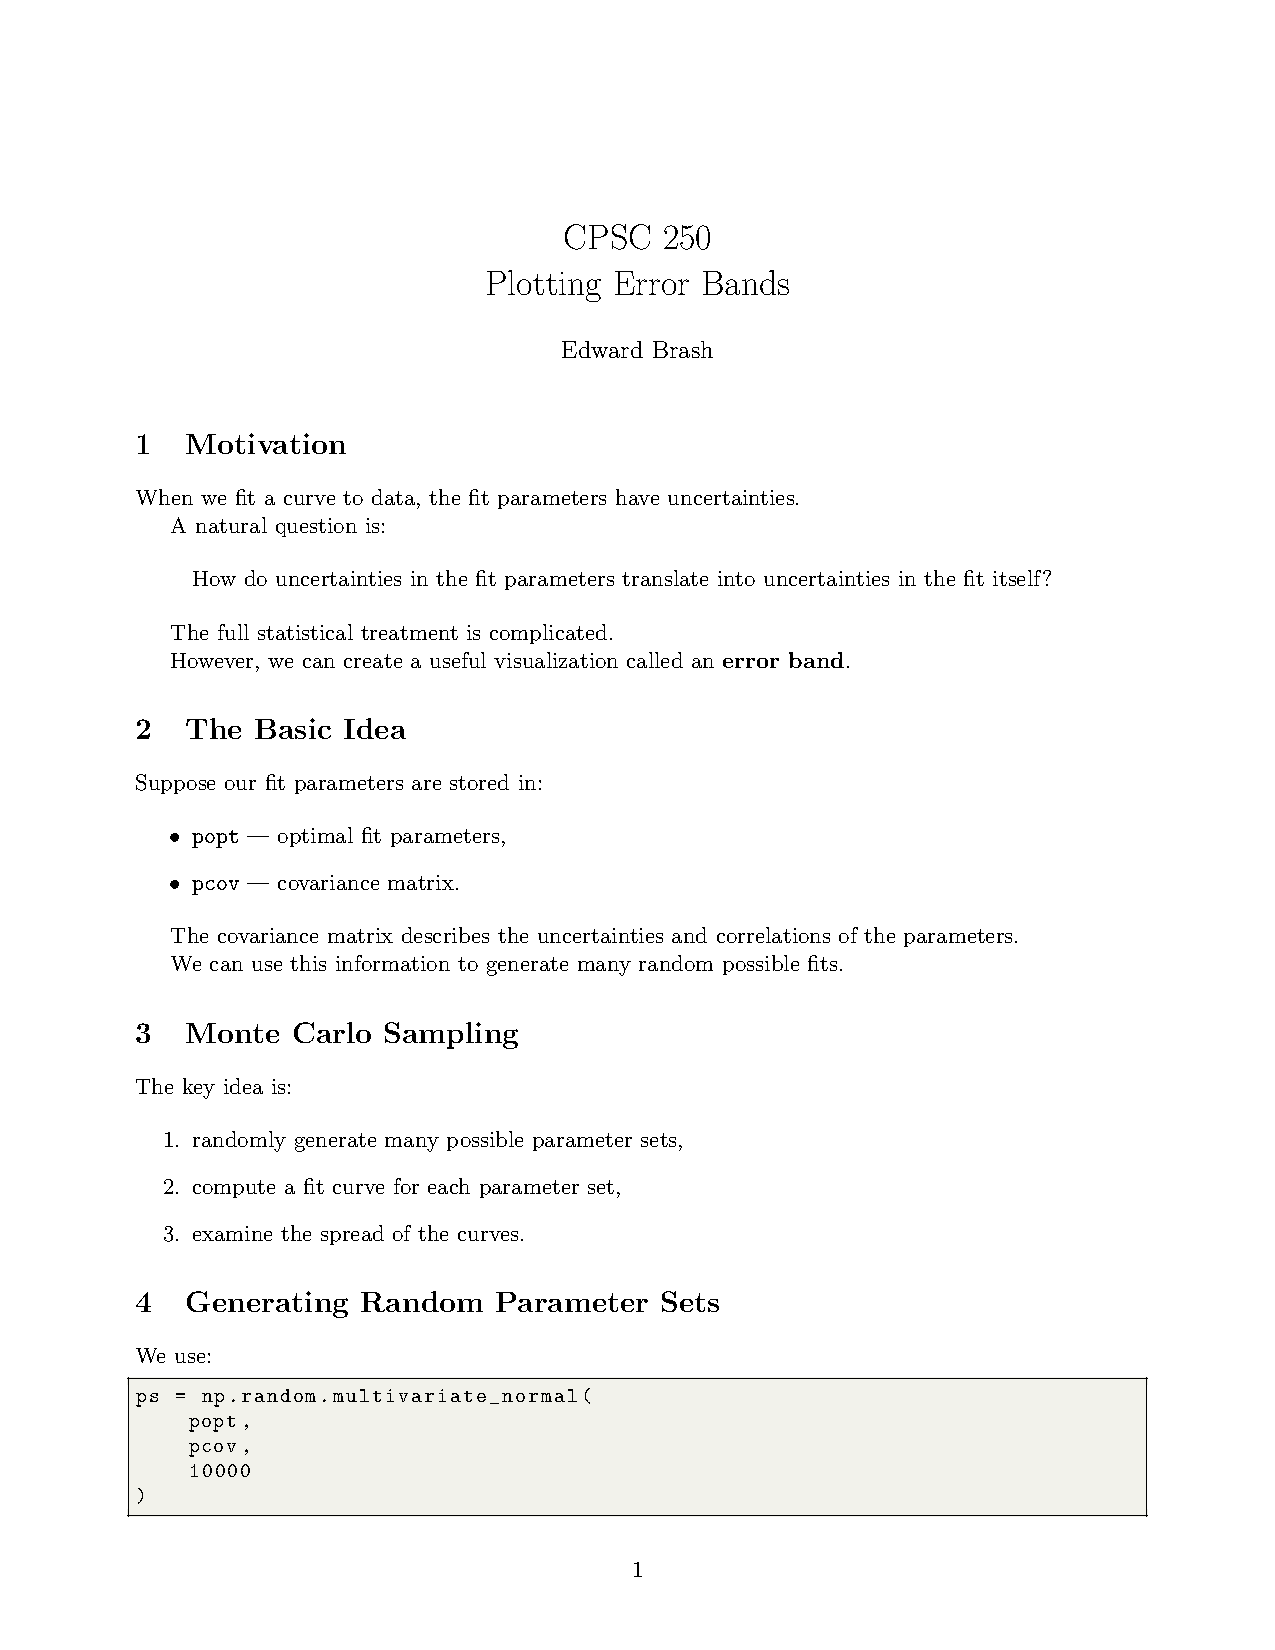
\includepdf[
    pages=-,
    addtotoc={1,subsection,2,{Plotting Error Bands},week4d}
]{Week4_Lectures/week4d_plotting_error_bands.pdf}

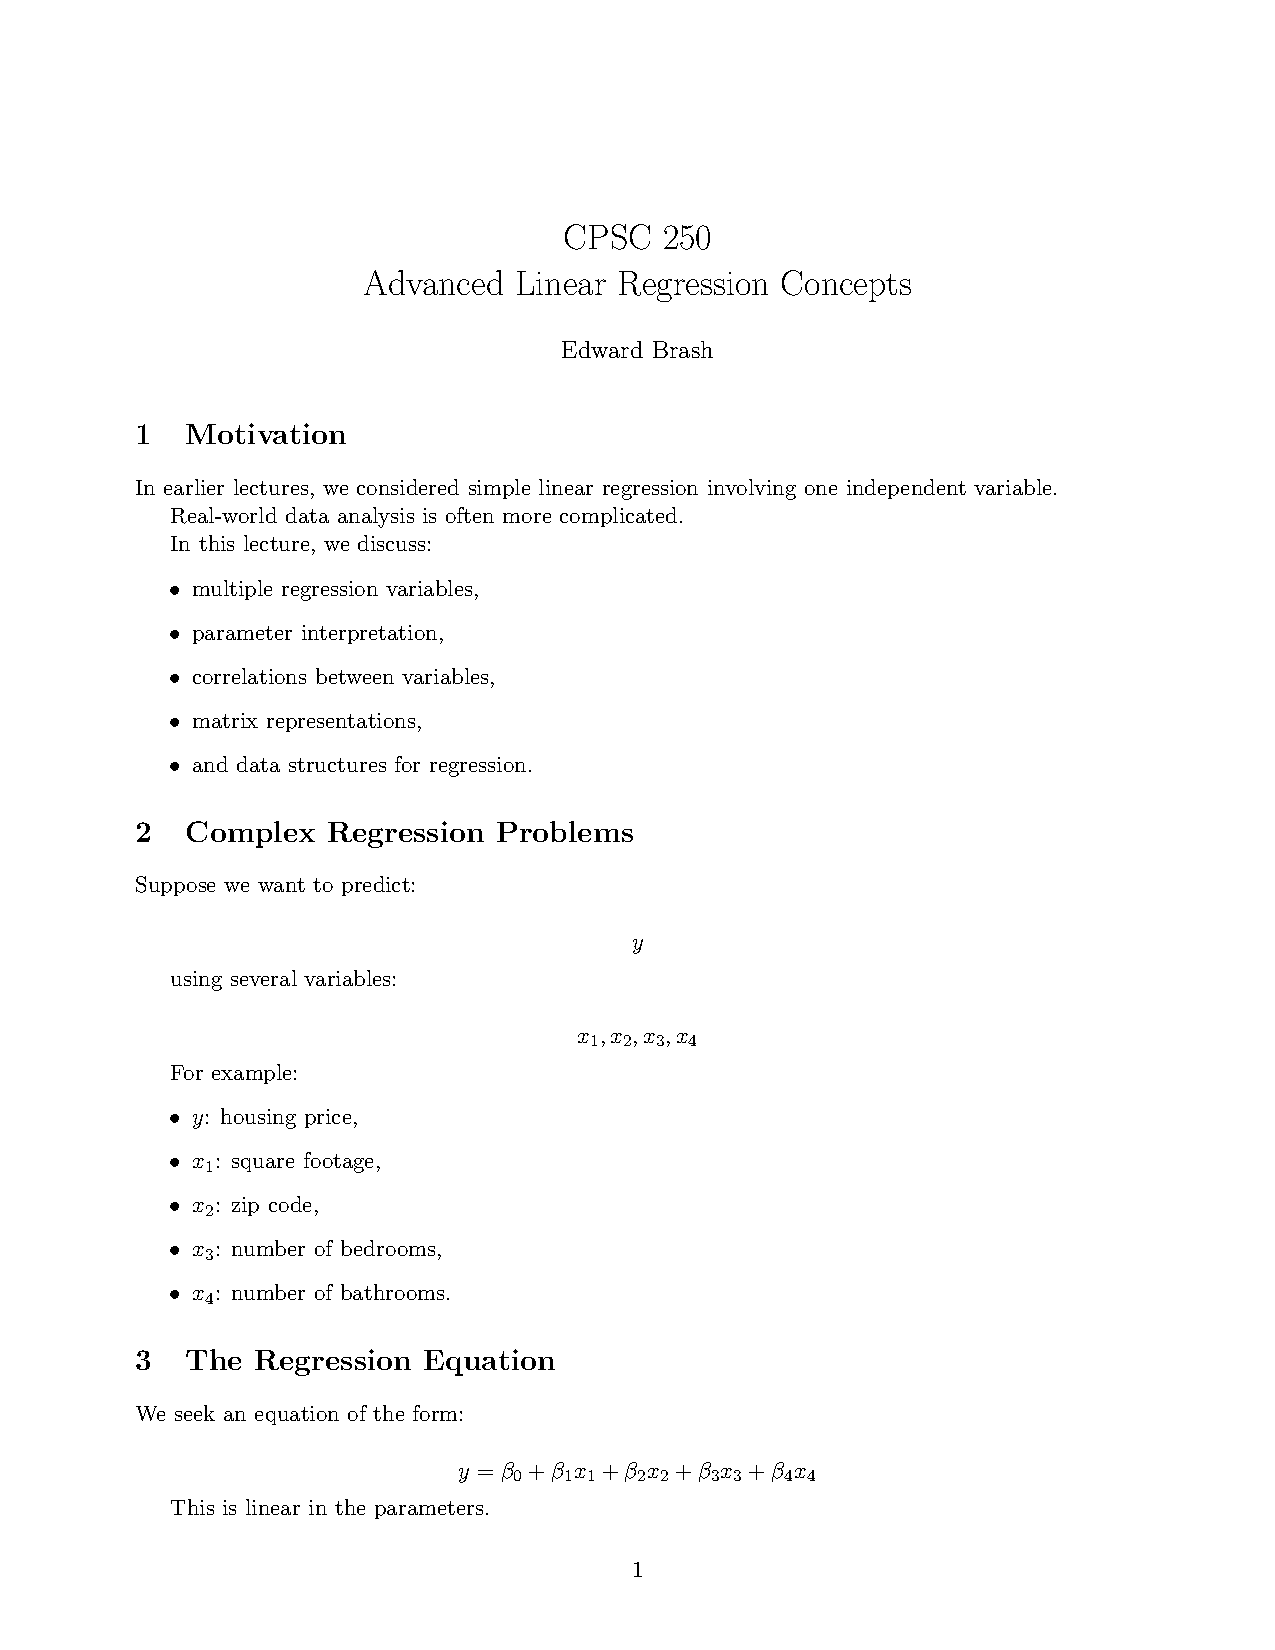
\includepdf[
    pages=-,
    addtotoc={1,subsection,2,{Advanced Linear Regression},week4e}
]{Week4_Lectures/week4e_advanced_linear_regression.pdf}

\includepdf[
    pages=-,
    addtotoc={1,subsection,2,{Git Command Summary},week4f}
]{Week4_Lectures/week4f_git_command_line_summary.pdf}

\end{document}
